\documentclass[a4paper, 11pt, oneside]{Thesis}

\usepackage[utf8]{inputenc}
\usepackage[T1]{fontenc}
\usepackage{lmodern}

\usepackage[square, numbers, comma, sort&compress]{natbib}

\usepackage{changepage}
\usepackage{float}
\usepackage[section]{placeins}

\usepackage{xcolor} 
\definecolor{rred}{HTML}{e0304e}

\lstset{
  captionpos=b,
  frame=tb,
  comment=[l]{\#},
  basicstyle=\ttfamily\footnotesize\linespread{1.2}\selectfont,
  numberstyle=\footnotesize\color{gray},
  commentstyle=\itshape,
  showstringspaces=false,
  keepspaces=true,
  aboveskip=2em,
  numbers=left,
  escapeinside={<@}{@>},
  moredelim=**[is][\color{rred}]{[@}{@]}
}

\usepackage[capitalise,noabbrev]{cleveref}
\crefname{sublstlisting}{Listing}{Listings}
\Crefname{sublstlisting}{Listing}{Listings}
\crefdefaultlabelformat{#2{\scshape #1}#3}
\AtBeginDocument{\DeclareCaptionSubType{lstlisting}}

\usepackage{varwidth}
\usepackage{verbatim}
\usepackage{stmaryrd}
\usepackage{mathtools}
\DeclarePairedDelimiter\set{\lbrace}{\rbrace}
\DeclarePairedDelimiter\bbrackets{\llbracket}{\rrbracket}
\DeclarePairedDelimiter\angles{\langle}{\rangle}
\DeclarePairedDelimiter\ttangles{\mathtt{<}}{\mathtt{>}}
\newcommand{\univ}{\ensuremath{\mathbb{U}}}

\usepackage{bussproofs}
\def\labelSpacing{1em}
\usepackage[altpo,epsilon]{backnaur}
\newcommand{\bnfmor}[1]{\bnfmore{\hspace{-1.5em}\ooalign{|\cr\hspace{1.5em}}#1}}

\usepackage{tipa}
\newcommand{\ipa}[1]{{\usefont{T3}{cmr}{m}{n}\selectfont#1}}

\usepackage{tikz}
\usetikzlibrary{chains,shapes,arrows,calc,positioning}
\tikzstyle{arrow} = [draw, -latex']
\tikzstyle{box} = [rectangle, draw=black!50, align=left, font={\ttfamily}]
\tikzstyle{init} = [circle, draw=black!50]
\tikzstyle{circ} = [circle, font={\ttfamily}]

\usepackage{siunitx}
\usepackage{csvsimple}
\usepackage{pgfplots}
\pgfplotsset{compat=1.18}
\usepackage{pgfplotstable}
\usepackage{xstring}
\pgfplotsset{where/.style 2 args={
    x filter/.code={
      \IfStrEq{\thisrow{#1}}{#2}{}{\def\pgfmathresult{}}
    }
  }
}

\usepackage{afterpage}
\usepackage{longtable}
\usepackage{amssymb}% http://ctan.org/pkg/amssymb
\usepackage{pifont}% http://ctan.org/pkg/pifont
\usepackage{comment}
\usepackage{algorithm}
\usepackage{algpseudocode}
\usepackage[newfloat]{minted}
\usepackage{physics}
\usepackage{caption}

\graphicspath{{figures/}}
\def\datapath{data}

\begin{document}

\frontmatter
\newcommand{\cmark}{\ding{51}}%
\newcommand{\xmark}{\ding{55}}%

%TC:macro \suhrid [ignore]
\newcommand{\suhrid}[1]{\textcolor{blue}{\textsc{Suhrid:} \textbf{#1}}\par}

%TC:macro \tawfiq [ignore]
\newcommand{\tawfiq}[1]{\textcolor{red}{\textsc{Tawfiq:} #1}\par}

%TC:ignore
\university{{The University of Melbourne}}
\UNIVERSITY{{THE UNIVERSITY OF MELBOURNE}}
\department{{School of Computing and Information Systems}}
\school{{Faculty of Engineering and IT}}
\degree{{Master of Computer Science}}
\title{{SLA-Driven Hybrid Autoscaling for Edge Computing}}
\shortauthors{{Suhrid Gupta}}
\authors{
  \texorpdfstring{\href{mailto:suhrid.gupta@student.unimelb.edu.au}{\shortauthornames}}{\shortauthornames}\\
  \small Student Number: 1313675
}
\supervisor{{Dr.~Rajkumar Buyya and Dr.~Muhammed Tawfiqul Islam}}
\addresses{\deptname\\\univname}
\date{June 2024}
\subject{}
\keywords{}
%TC:endignore

%TC:envir lstlisting [option:text] xall
%TC:ignore
%\wordcount{\input{|"bash ./Scripts/FMT-TexCount \jobname.tex"}}
%TC:endignore

\maketitle

\setstretch{1.3}

\fancyhead{}
\rhead{\thepage}
\lhead{}

\pagestyle{fancy}

%TC:ignore
%\quotepage{
%If you aren't sure which way to do something,\\
%do it both ways and see which works better.
%}{
%John Carmack
%}

%\addtotoc{Abstract}  % Add the "Abstract" page entry to the Contents
\abstract{
\addtocontents{toc}{\vspace{1em}}  % Add a gap in the Contents, for aesthetics

Edge computing decentralizes computing resources, allowing for novel applications in domains such as the Internet of Things (IoT) in healthcare and agriculture by reducing latency and improving performance. This decentralization is achieved through the implementation of micro-service architectures, which require low latencies to meet stringent service level agreements (SLA). While cloud computing offers the large data storage and computation resources necessary to handle peak demands, a hybrid cloud and edge environment is required to ensure SLA compliance. This is achieved by sophisticated orchestration strategies such as Kubernetes, which help facilitate resource management. The orchestration strategies alone do not guarantee SLA adherence due to the inherent delay of scaling resources. Existing auto-scaling algorithms have been proposed to address these challenges, but they suffer from performance issues and configuration complexity. In this thesis, a novel auto-scaling algorithm is proposed for SLA-constrained edge computing applications. This approach combines a Machine Learning (ML) based proactive auto-scaling algorithm, capable of predicting incoming resource requests to forecast demand, with a reactive autoscaler which considers current resource utilization and SLA constraints for immediate adjustments. The algorithm is integrated into Kubernetes as an extension and its performance is evaluated through extensive experiments in an edge environment with real applications. The results demonstrate that existing solutions have an SLA violation rate of up to 17\%, whereas the proposed hybrid solution outperforms the baselines and has an SLA violation rate of 6\%, ensuring stable SLA compliance across various applications.

}
%
% Guidelines as of 2019/06/04
% https://gradresearch.unimelb.edu.au/__data/assets/pdf_file/0004/2027839/Preparation-of-GR-theses-rules.pdf
%
\Declaration{

I, \shortauthornames, declare that this thesis titled, ``Enhanced SLA Compliance in Edge Computing Applications through Hybrid Proactive-Reactive Autoscaling'' and the work presented in it are my own. I confirm that:

\begin{itemize} 
\item[\tiny{$\blacksquare$}] this thesis does not incorporate without acknowledgement any material previously submitted for a degree or diploma in any university; and that to the best of my knowledge and belief it does not contain any material previously published or written by another person where due reference is not made in the text.

\item[\tiny{$\blacksquare$}] this thesis did not require clearance from the University's ethics committee.

\item[\tiny{$\blacksquare$}] the thesis is approximately \num[group-separator={,}]{24000} words in length (excluding text in figures, tables, code listings, bibliographies, and appendices).

\end{itemize}
}
{}
\clearpage
%
% Guidelines as of 2019/06/04
% https://gradresearch.unimelb.edu.au/__data/assets/pdf_file/0004/2027839/Preparation-of-GR-theses-rules.pdf
%
\Preface{
Section~\ref{subsec:ch2-k8s-overview} of the thesis which provides an overview of Kubernetes was modified from the research proposal that was undertaken in partial fulfillment of the requirements of the \degreename.\par
All work written by myself in support of this thesis was independently reviewed by my supervisors, \supname. Feedback was also received from my supervisors throughout the creation of the thesis and was incorporated into the final version.

\hiddensection{Publications}
\begin{table}[h!]
    \centering
    \begin{tabular}{p{3cm}p{6cm}p{4cm}}
        \toprule
        \textbf{Authors} & \textbf{Title} & \textbf{Venue}\\
        \midrule
        \multirow{2}{3cm}[-3em]{Suhrid~Gupta, Tawfiq~Islam, Rajkumar~Buyya} & SLA-Driven Hybrid Autoscaling for Edge Computing: Foundations, Review, and Future Directions & ACM Computing Surveys (in submission)\\\\
         & A Hybrid Reactive-Proactive Autoscaling Approach for Microservice Applications in Edge Computing Environments & Journal of Systems and Software (in submission)\\
        \toprule
    \end{tabular}
\end{table}

}
\clearpage
\acknowledgements{
\addtocontents{toc}{\vspace{1em}}  % Add a gap in the Contents, for aesthetics

I wish to thank my primary supervisor, Dr. Tawfiq Islam for his generous and invaluable support, feedback, patience, and guidance throughout the whole research process. His continuous encouragement and insights, both personal and professional, has made an immeasurably impact on me throughout my two semesters working under his supervision. I further wish to thank my co-supervisor Prof. Rajkumar Buyya. His guidance in helping me to set up milestones ensured I met my research deadlines. I am grateful to have had them both as my supervisors, and this research thesis would not have been possible without their support.\par

I further wish to thank my friends and family for their selfless help and constant support throughout my time here at The University of Melbourne, for always motivating me, and for their endless guidance which has helped me complete this research project.\par

}

\tableofcontents
\listoffigures
\listoftables
\lstlistoflistings
\listofalgorithms
%TC:endignore

\addtocontents{toc}{\vspace{1em}}

\mainmatter	
\pagestyle{fancy}
\setstretch{1.5}

\clearpage

\def\chaptertitle{Introduction}

\lhead{\emph{\chaptertitle}}

\chapter{\chaptertitle}
\label{ch:introduction}

In this chapter, a brief overview of the edge computing architecture paradigm, along with its uses, benefits, and challenges with respect to resource scaling are provided in section \ref{sec:edge-arch}. These challenges lead to the research gap and questions this thesis intends to answer in section \ref{sec:problem-overview}.\par

\section{Edge Computing Overview}
\label{sec:edge-arch}

Cloud computing architectures leverage the on-demand accessibility of the Internet. The cloud applications utilize the vast resources of the cloud to perform a task, and relinquish it once it is complete for the other sub-modules in the application to request \cite{rimal2009taxonomy}. In the early days, a singular end-point would be used to access these services, however nowadays the architecture is multi-regional allowing effortless access from across the world. This was achieved through the use of content delivery networks (CDN) located in several regions to allow for data to be quickly replicated and served to clients. This architecture model allows for the processing of large-scale data in a near real-time manner.\par

During the early twenty-first century, this architecture paradigm dominated the Information Technology (IT) industry. Compared to traditional monolithic architectures, the ease of deployment, scalability, coupled with the economic benefits ensured its dominance. The increasing popularity of hand-held devices as well as home appliances has resulted in data being largely produced at the edge of the cloud network. Thus, processing this large amount of data solely on the cloud proved to be an inefficient solution due to the bandwidth limitations of the network \cite{shi2016edge}. Thus, edge computing paradigms were built on the previous foundation of CDNs \cite{satyanarayanan2017emergence}. Edge computing architectures ensure data processing services and resources exist at the peripheries of the network \cite{cao2020overview}. The architecture extends and adapts the computing and networking capabilities of the cloud to meet real-time, low latency, and high bandwidth requirements of modern agile businesses.\par

Edge computing deploys several lightweight computing devices known as cloudlets to form a ``mini-cloud'' and places them in close proximity to the end-user data \cite{liu2019survey}. This reduces the latency in terms of client-server communication and data processing. Figure \ref{fig:edge-architecture-overview} shows a high-level overview of this architecture. Cloudlets can also be easily scaled depending on the resource requirements per edge architecture \cite{ren2019survey}. However, due to the dynamic resource requirements which may fluctuate from time to time, the resources allocated to cloudlets must be dynamically scaled too. This dynamic scaling, along with the inherent latency present between the cloud layer and the edge cloudlets, poses a significant problem to real-time resource scaling \cite{varghese2016challenges}.\par

\begin{figure}[htb]
    \centering
    \caption{Overview of edge computing architecture}
    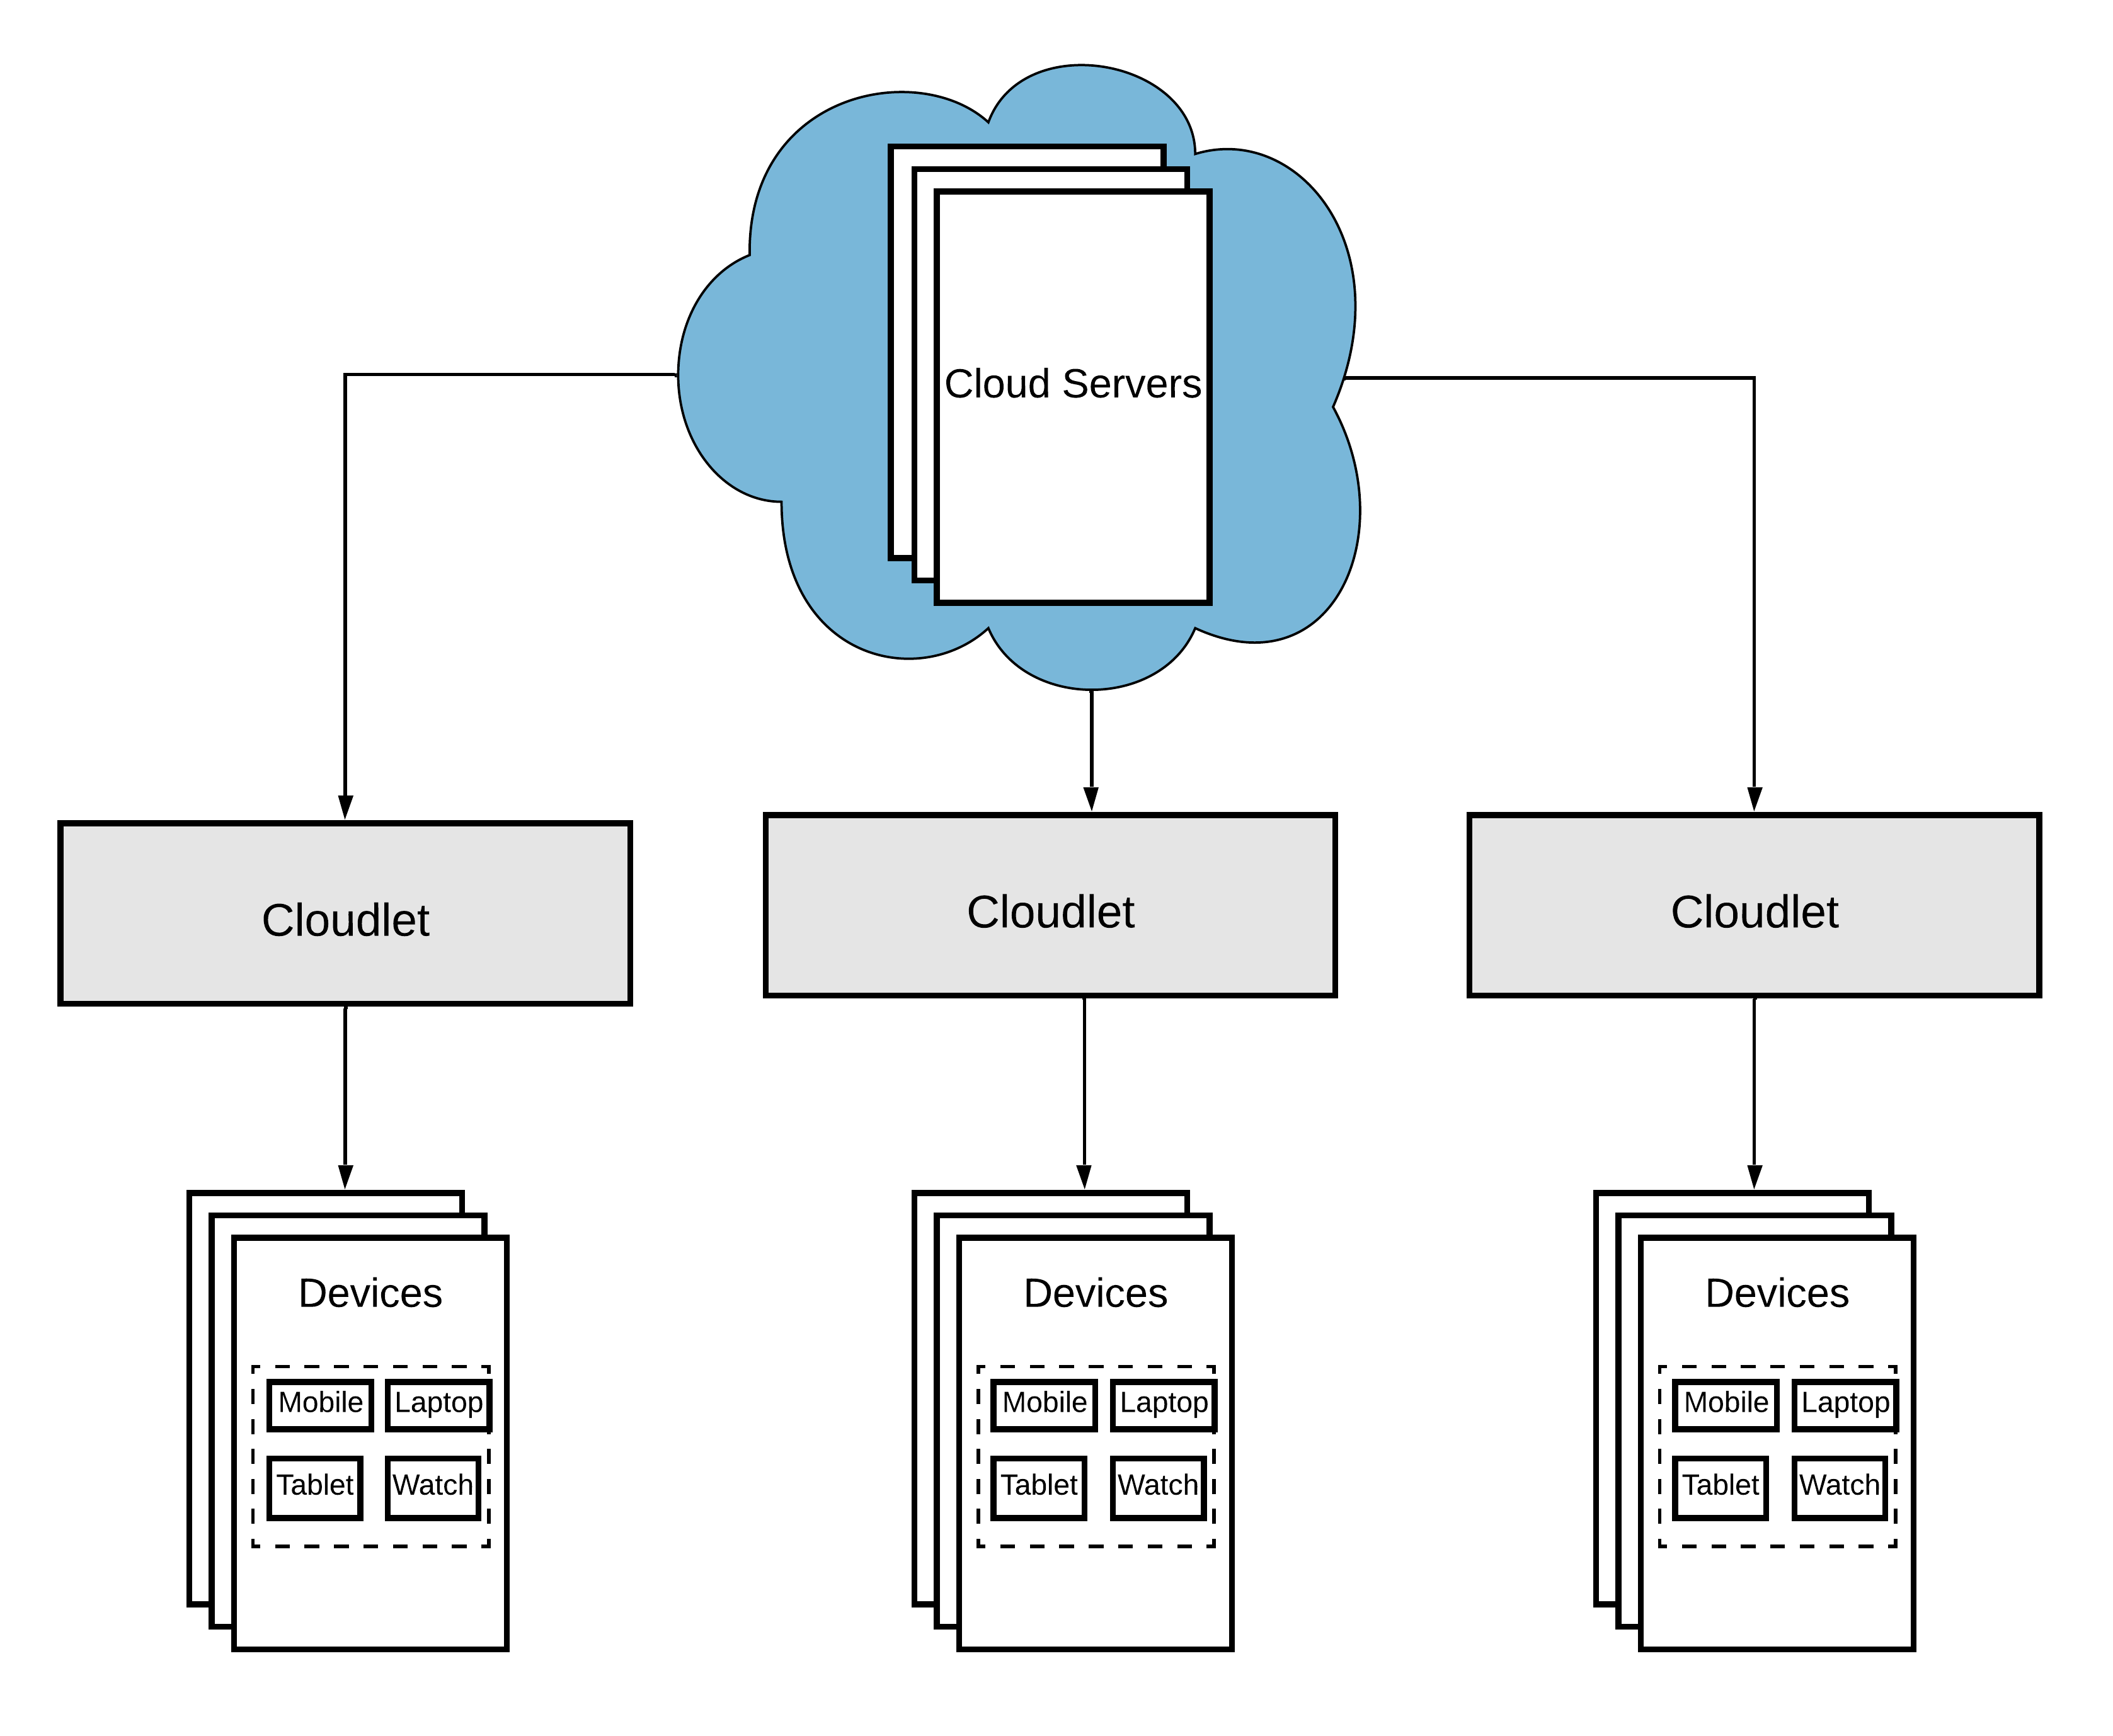
\includegraphics[width=0.9\linewidth]{Figures/Edge-Architecture-Overview.png}
    \label{fig:edge-architecture-overview}
\end{figure}

One method of mitigating this scaling latency is through the use of micro-service applications. By employing a microservice architecture, the resources in a cloudlet are a collection of smaller deployments that are both independent and loosely coupled \cite{villamizar2015evaluating}. This loose coupling ensures that parts of the cloudlet can be scaled as is required, further reducing the time required to scale resources as compared to scaling the cloudlet monolithically.\par

The scaling of these microservice resources is done automatically through a process known as autoscaling. While most microservice applications come bundled with default autoscaling solutions, and these solutions are sufficient for most applications, they fall apart when scaling resources for time-sensitive services such as the ones used in healthcare require stringent compliance to service level agreements (SLA) on metrics such as application latency. This has led to further research on autoscaling solutions for edge computing applications. These primarily fall into two categories. Reactive autoscaling solutions attempt to modify the microservice resource allocation once the required resources exceeds the current allocation. These algorithms are simple to develop and deploy, however the time taken to scale resources leads to a degradation of resource availability and violates SLA compliance \cite{podolskiy2018iaas}. To counteract these pitfalls, proactive autoscaling solutions attempt to model the resource allocation over time and effectively predict the resource requirements. By doing so, the microservice resources can be scaled in advance through a process known as ``cold starting''. This approach removes the latency inherent in scaling resources, however the algorithms are extremely complex to develop, train as well as tune to specific edge applications \cite{straesser2022not}.

\section{Problem Overview}
\label{sec:problem-overview}

With these limitations in mind, the object of this research project was to unify the reactive and proactive autoscaling solutions into a hybrid model. This solution combines the light weight, and ease of use and deployment of the reactive algorithm, with the SLA compliance and accurate resource modelling of proactive ones. The project aimed to answer the following questions in a satisfactory manner:
\begin{itemize}
    \item \textbf{\textit{RQ1:}} Can we integrate reactive and proactive autoscaling methods to develop a tailored algorithm for edge computing that eliminates the requirement for developers to fine-tune hyper-parameters for each autoscaling use case, while being lightweight enough to be deployed and run on cloudlets?
    \item \textbf{\textit{RQ2:}} Can the hybrid autoscaling solution achieve or exceed the SLA compliance capabilities of state-of-the-art reactive and proactive autoscaling solutions for edge computing, while minimizing the degredation of application performance?
\end{itemize}
\clearpage

\def\chaptertitle{Background}

\lhead{\emph{\chaptertitle}}

\chapter{\chaptertitle}
\label{ch:background}

In this chapter, a brief introduction to Service Level Agreements is provided in section \ref{sec:sla}, followed by an overview of microservice architectures is provided in section \ref{sec:micro-svc-arc}. This includes a brief description of the architecture of Kubernetes, along with its scheduling and autoscaling algorithms. Finally, section \ref{sec:lit-review} comprises of a detailed literature review of the state-of-the-art autoscaling algorithms and a comparison of their performances and drawbacks.

\section{Service Level Agreements}
\label{sec:sla}

\begin{figure}[htb]
    \centering
    \caption{Types of service level agreements}
    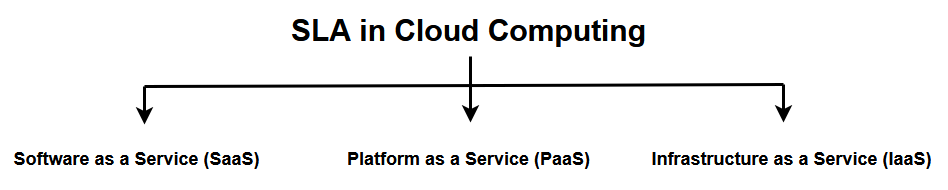
\includegraphics[width=0.9\linewidth]{Figures/SLA-Cloud-Computing.png}
    \label{fig:sla-types}
\end{figure}

Cloud computing generally exposes resource using a pay-as-you-go service. These lucrative plans have led to the implementation of applications and hardwares being delivered as Software as a Service (SaaS), Platform as a Service (PaaS), and Infrastructure as a Service (IaaS). However, consumers of such services have demands which may vary significantly, and it is impossible to fulfill all these expectations. Thus a balance needed to be struck in order to commit to an agreement \cite{patel2009service}. \par
This commitment is known as a Service Level Agreement (SLA). This SLA defines the expected services provided by the provider, and agreed to by the consumer. The most common metric by which SLAs are negotiated between providers and consumers is the availability of service.

\subsection{Availability of Services}
\label{subsec:svc-availability}
Availability is defined to ensure that the functional performance of the edge deployment is maintained for an agreed period. SLAs mostly define either monthly or yearly downtime in order to compute service credits for billing purposes \cite{mirobi2015service}. The downtime can be calculated using the formulae:
%TC:ignore
\[ downtime_{monthly} = \frac{100 - Availability\%}{100} * 30 * 24 \]
\[ downtime_{yearly} = \frac{100 - Availability\%}{100} * 365 \]
%TC:endignore
Table \ref{table:sla-availability} shows the expected down-times for several SLA availability percentages.

%TC:ignore
\begin{table}
    \caption{Summary of SLA availability}\label{table:sla-availability}
    \centering
    \begin{tabular}{|l|l|l|}
        \hline
        Availability \% & Monthly Downtime & Yearly Downtime\\
        \hline
        90\% & 72 hours & 36.5 days\\
        99\% & 7.2 hours & 3.65 days\\
        99.9\% & 43.8 minutes & 8.76 hours\\
        99.99\% & 4.38 minutes & 52.56 minutes\\
        99.999\% & 25.9 seconds & 5.26 minutes\\
        \hline
    \end{tabular}
\end{table}
%TC:endignore

\section{Microservice Architecture}
\label{sec:micro-svc-arc}

Microservice architectures involve decomposing an application into several loosely coupled services, and deploying them on separate servers known as ``nodes''. These services communicate with each other through a lightweight framework such as RESTful APIs \cite{li2021understanding}. Within these services, application data and commands are stored and executed within ``containers''. Typically, these architectures provide scalability, as well as ease of deployment and modification. Availability however, remains an important concern for such deployments. For a deployment to be classified as ``highly available'', it must be accessible at least 99.999\% of the time. For example, a highly available search engine would only face 5 minutes of down time per year \cite{nabi2016availability}. Therefore, an orchestration mechanism is required to manage the deployment and communication of these containers.\par

\begin{figure}[htb]
    \centering
    \caption{Features of Container Orchestration}
    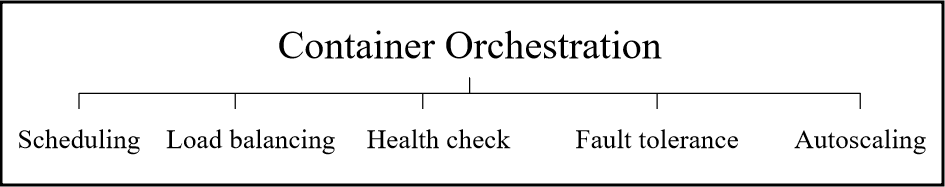
\includegraphics[width=0.9\linewidth]{Figures/Container-Orchestration.png}
    \label{fig:container-orchestration}
\end{figure}

Container orchestration allows the microservice application to customize how the deployment, monitoring, and controlling functions \cite{casalicchio2019container}. Figure \ref{fig:container-orchestration} depicts the typical features of container orchestration.\par
\textit{Scheduling} defines the rules on the number of containers to be executed at any given time. Scheduling also places containers on specific nodes based on availability and best performance.\par
\textit{Load balancing} distributes the resource usage among multiple microservice nodes. By default, a round-robin policy is implemented, although more complex policies may be implemented at the discretion of the developer.\par
\textit{Health checks} ensure that the container is still capable of responding to queries. Typically, these are done using a periodic light-weight HTTP request and verifying the response.\par
\textit{Fault tolerance} maintains several replicas of containers, a strategy commonly used to achieve the high availability mentioned above. Health checks are used to ensure the replicas are functioning, and they typically have strategies to ensure there is no mismatch in data between two fault tolerant containers.\par
\textit{Autoscaling} is the process of automatically adding or removing resources or containers. Internal metrics such as CPU usage are typically used, however custom policies can also be implemented at the discretion of the developer.\par

\subsection{Kubernetes Architecture}
\label{subsec:k8s-overview}

Kubernetes \footnote{\url{https://kubernetes.io/}} is one of the most popular open-source container orchestration platforms \cite{vayghan2019kubernetes}. Initially referred to as ``Borg'', the project was used internally at Google to deploy the majority of their cloud applications before becoming an open-source application \cite{burns2016borg}. Figure \ref{fig:k8s-arch} shows the high-level architecture. The Kubernetes deployment has a controller / worker architecture. The nodes in the Kubernetes cluster are split into either \textit{control plane nodes} and \textit{data plane nodes}. The \textit{control plane nodes} have a collection of processes which help monitor and maintain the desired state of the deployment. The \textit{data plane nodes} contain processes which run the containers doing the actual work, and are managed by the control plane.\par
The smallest unit of work in a Kubernetes deployment is known as a \textit{pod} \cite{baier2017getting}. This is a collection of containers sharing an IP address and port. In summary, microservice architectures are said to be containerized and deployed on Kubernetes in the form of pods \cite{vayghan2019kubernetes}.\par
\begin{figure}[htb]
    \centering
    \caption{Kubernetes Architecture}
    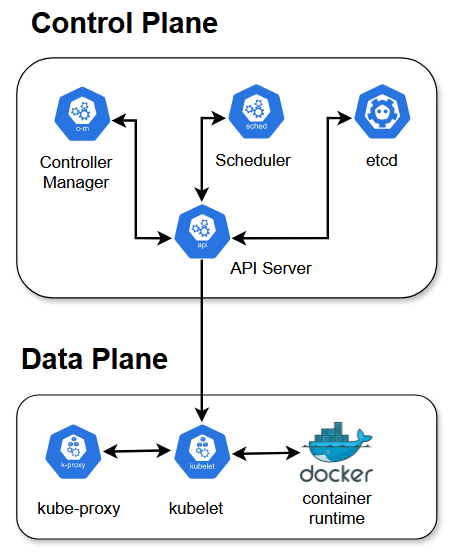
\includegraphics[width=0.5\linewidth]{Figures/K8s-Architecture.png}
    \label{fig:k8s-arch}
\end{figure}

\subsubsection{Data Plane}
\label{subsubsec:k8s-data-plane}

The \textit{container runtime} is a process which downloads or ``pulls'' the image for the required container onto the node. Kubernetes supports a wide range of runtimes, but some of the popular solutions are CRI-O \footnote{\url{https://cri-o.io/}}, containerd \footnote{\url{https://containerd.io/}}, and Docker \footnote{\url{https://www.docker.com/}}.\par

The most important process running on every data plane node is the \textit{kubelet}. This process executes the image assigned to the node via the container runtime, perform health checks, and reports the node status to the control plane.\par

Another data plane process is the \textit{kube-proxy}, which manages the rules for forwarding requests to services, as well as the IP tables of nodes. If a service is added or removed, kube-poxy updates the IP table accordingly.\par

\subsubsection{Control Plane}
\label{subsubsec:k8s-control-plane}
The \textit{API Server} is the primary communication endpoint for the entire deployment. Every component in the architecture communicates through it to exchange information. It is also used to update the current deployment state. The API Server is a simple RESTful API implementation, exposing well-documented APIs for access by other components as well as developers. Multiple replicas of this component are typically maintained to ensure high availability.\par

The \textit{etcd} is a data store which persists the deployment state in a key-value format. The data is serialized unlike in the stateless API server. This data adheres the properties of \textit{recovery} and \textit{availability}. \textit{Recovery} ensures that any corruption of data is reverted using a system of backups such as checkpoints. \textit{Availability} ensures that the deployment is reachable by the end-user regardless of the traffic being requested on the network.\par

\textit{Controller Manager} implements the desired deployment state. During initial deployment, the controller manager inputs the required workload as the desired state, after which it continually monitors the deployment state using a system of looping controls. If the deployment requires modifications, they are achieved using the API server, and the deployment is brought back into alignment with the desired state.\par

Finally, the \textit{scheduler} decides the location where the pod will be deployed. The scheduler runs a control loop which searches for uncheduled pods using the API server. It then assigns the pods to a dataplane node based on several predicates and priorities such as resource requirements and node affinity respectively.

\section{Autoscaling Overview}
\label{sec:autoscaling}

Apart from intelligently scheduling pods to data plane nodes \cite{kayal2020kubernetes}, Kubernetes has the provisions to dynamically respond to changes in resource requirements. This process of scaling nodes, pods, or other resources depending on requirements in an automated manner is known as \textit{autoscaling}. Kubernetes supports three variations of autoscaling.\par

\textit{Cluster autoscaling} modifies the number of nodes running in the entire deployment, or cluster. Dynamically allocating nodes based on resource requirements helps to manage the cost of running Kubernetes deployments on external platforms such as Amazon \footnote{\url{https://docs.aws.amazon.com/eks/}} or Google \footnote{\url{https://cloud.google.com/kubernetes-engine/}}. The autoscaler works by looping through two tasks. The first watches for unscheduled pods, the second checks if the current deployed pods (pods which are running on the data plane) can be merged on a smaller number of nodes.\par

\textit{Vertical pod autoscaling} modifies the CPU and memory resources assigned to pods. By default, the scheduler reserves a larger amount of these resources to pods than is usually required. By performing vertical pod autoscaling, the cluster can better manage its over-provisioned resources in real-time.\par

\textit{Horizontal pod autoscaling} is the most commonly used autoscaling strategy \cite{baresi2021kosmos}, it modifies the number of pods assigned to a task, based on the resources being requested. Kubernetes implements this using a periodic control loop which runs every 15 seconds by default. The control manager compares the actual resource utilization with the target utilization defined by the deployment script, and scales the number of pods accordingly.

\subsection{Custom Autoscaling}
\label{subsec:custom-autoscaling}

The default horizontal pod autoscaler uses pod CPU and memory utilization when making its scaling decisions. However, these metrics may be too rigid when it comes to edge architectures \cite{coulson2020adaptive}. The strict SLA constraints in place, along with the lower amount of resources present in the edge layer as compared to the cloud layer, make it imperative for custom metrics to be employed to autoscale resources as efficiently as possible.\par

Figure \ref{fig:custom-autoscale-overview} depicts the general architecture of the custom autoscaler. Typically, the autoscaler queries metrics from the default metrics registry, which acts as a central store for all metrics that are exposed to the developer. Three interfaces to this registry are exposed:
\begin{itemize}
    \item \textit{Resource metric API} is used to access predefined metrics such as CPU and memory resources of both pods as well as nodes.
    \item \textit{Custom metric API} contains user-defined custom metrics associated with all Kubernetes objects.
    \item \textit{External metrics API} contains metrics of objects which are not associated with Kubernetes.
\end{itemize}
For custom metric autoscaling, the autoscaler must be configured in a way where the metrics can be fetched from the custom metric API. This is done by configuring the custom metric server, several frameworks to simplify this process such as the Kubernetes Instrumentation SIG \footnote{\url{https://github.com/kubernetes/community/tree/master/sig-instrumentation}} exist which simplify the server building process.

\begin{figure}[htb]
    \centering
    \caption{Custom Autoscaler Architecture Overview.}
    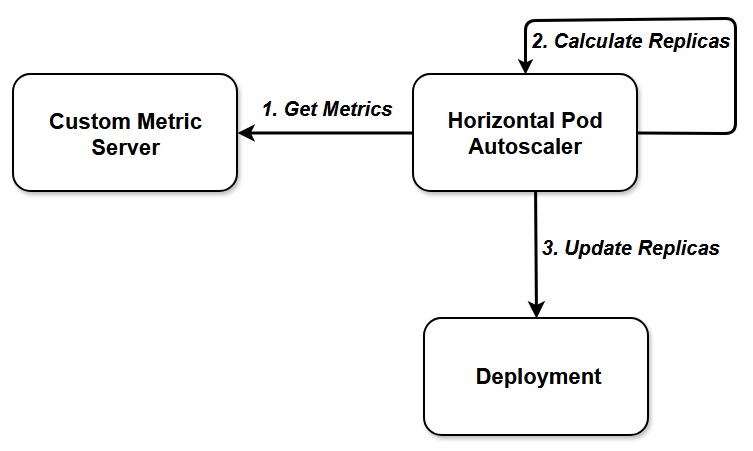
\includegraphics[width=.7\linewidth]{Figures/Custom-Metrics-Autoscaling.png}
    \label{fig:custom-autoscale-overview}
\end{figure}

\section{Literature Review}
\label{sec:lit-review}

In this section, we discuss some of the common challenges and limitations inherent in an edge computing paradigm, before delving into the many attempts at mitigating them.

\subsection{Edge Computing Issues and Challenges}
\label{subsec:edge-issues}

\subsubsection{Resource Allocation}
\label{subsubsec:edge-resource-alloc}

Cao et al. \cite{cao2020overview} demonstrated the key differentiations traditional cloud computing architectures have compared to edge architectures, while asserting that edge deployments remain an extension of the cloud. The aim of cloud computing infrastructures is to process huge amounts of data from multi-regional zones, or in the best case, globally. This is done so as to perform in-depth analysis in diverse fields such as health-care, robotics, and business decision making. Traditionally, they also dealt with non-real-time data for decision-making \cite{premsankar2018edge}. On the other hand, edge computing usually handles smaller scale data, locally clustered and isolated in separate zones, and highly real-time in nature \cite{mishra2020early}. The data processed in traditional cloud computing environments are also generally done using a high network bandwidth. This is due to the large distances data needs to be transmitted over to reach the data centres and cloud servers. Such data transmission places an enormous burden on the cloud network, and poses multiple security challenges in ensuring that the data is not compromised in transit.\par

The real-time nature of edge computing applications necessitates a method of resource allocation which ensures minimal cost of deployment, and maximum efficiency in terms of performance. As mentioned in section \ref{sec:edge-arch}, micro-service container orchestration technologies are leveraged to achieve these aims. Kristiani et al. \cite{kristiani2019} demonstrated an edge computing architecture, where the edge layer consists of Kubernetes nodes. Such a deployment increases the scalability, as well as maintains the ease of deployment, upgrade, and removal of nodes in the edge layer. Scaling of resources through the means of autoscaling depending on the resource requirements is crucial to the architecture's performance. Default solutions such as the inbuilt autoscaler provided by Kubernetes, while generally useful for cloud applications, are unsuitable for edge architectures according to Phan et al. \cite{phan2022traffic}. They note that due to the algorithm's default nature to allocate resources in a round-robin manner, they do not take into account which Kubernetes nodes require resources the most, violating edge architecture paradigms.

\subsubsection{Cold start problem}
\label{subsubsec:cold-start}

To explain the cold start problem, we use the example of horizontal pod autoscaling in Kubernetes. When the control plane requests for a deployment to be scaled up, Kubernetes adds more pods to the dataplane nodes.  Based on the internal workload, the pod needs to be elastically scaled out \cite{beni2021reducing}. Even though the pod start up time is significantly quicker than, say, a traditional virtual machine, there is a latency inherent to bootstrapping the container, preparing the pod environment based on the deployment specification, and initialising the code present in the container image, and registering the pod in a ``ready'' state to the Kubernetes control plane. This latency inherent when scaling resources is known as the ``cold start''.\par

Several techniques exist to reduce this cold start latency. The Kubernetes container runtime uses snapshots \cite{cadden2019seuss}, lazy fetching of container images \cite{lorenzo2019fogdocker}, and container queues \cite{lin2019mitigating}. However, these measures do not eliminate the issue of cold start. Due to this, researchers looked into scaling resources in a predictive manner, so as to ensure the microservice application has enough time to spool up resources before the actual demand comes in.\par

\subsubsection{Service Level Agreements}
\label{subsubsec:sla-edge}

There are several challenges posed in providing SLA guarantees in an edge deployment:
\begin{itemize}
    \item Users queueing for large periods of time to use a service \cite{venticinque2011cloud}
    \item Degradation of application performance due to peak levels of workload, leading to user dissatisfaction \cite{sakr2012sla}
    \item Incorrect resources being allocated to the application, leading to either a degradation of availability, or large cost of application deployment \cite{houlihan2014auditing}
\end{itemize}

Several strategies have been proposed to counteract these challenges. Linlin et al. \cite{wu2013sla} proposed a customer-driven strategy  to minimize the provisioning costs. The algorithm considers the customer profiles as well as cloud providers' quality parameters such as response time to dynamically handle customer requests. Rajkumar et al. \cite{rajavel2012achieving} proposed a solution for alleviating the issue of delay in service allocation to users through the use of a novel hierarchical scheduling algorithm. This algorithm increases the performance of the scheduling algorithm, thus reducing the wastage of resources, and minimizing wait times. Sakr et al. \cite{sakr2012sla} introduced a novel approach to combat application performance degradation by using a middleware between consumers and the cloud. This middleware helps to facilitate dynamic provisioning of cloud databases based on consumer requirements, tailoring their needs and requirements to mitigate peak usages being hit often.

\subsection{Resource Management and Scheduling Solutions}
\label{subsec:resource-schedule-solutions}

To counteract the limitations discussed in section \ref{subsubsec:edge-resource-alloc}, several custom scheduling and resource management algorithms have been proposed for edge architectures.\par

Skarlat et al. \cite{skarlat2016resource} demonstrated an algorithm for resource scheduling where the usage of resources was formalized as an optimization problem. Thus, the authors attempted to minimize the network delay when requesting computational resources. Based on this work, Aazam and Huh \cite{aazam2015dynamic} proposed another solution for resource management which attempted to estimate the resources per service required, based on the user's previous behaviour as well as type of service being requested. By following such an approach, the resource wastage was actively reduced in edge nodes. Another resource allocation solution provided by Ni et al. \cite{ni2017resource} was based on priced timed Petri nets. The resources in the edge nodes are divided into several groups. The users can then select resources as per their requirements in an autonomous manner according to the price and time-cost of the operation.\par

Based on these initial proposals, Nguyen et al. \cite{nguyen2020elasticfog} revealed ElasticFog, a resource provisioning algorithm which operates on top of the Kubernetes architecture. The algorithm provides real-time elastic scheduling for the resources on the edge nodes by monitoring the traffic distribution on the network, thereby achieving a significantly higher throughput and network efficiency in comparison to the default Kubernetes scheduler solution.\par

Wojciechowski et al. \cite{wojciechowski2021netmarks} proposed a similar extension to the Kubernetes scheduler which deployed traffic-aware provisioning of resources. The extension worked alongside the Istio Service Mesh \footnote{\url{https://istio.io/latest/about/service-mesh/}} to collect dynamic network metrics for the scheduling of resources. The algorithm was shown to have highly efficient uses for edge deployments such as the 5G network.\par

While these proposals improved the scheduling and resource provisioning of edge deployments, they did not address key limitations addressed above such as the need for dynamic resource scaling so as to face the challenges of real-time data processing and SLA compliance. Due to these issues, several autoscaling algorithms were proposed to address them.

\subsection{Reactive Autoscaling Solutions}
\label{subsec:reactive-solutions}

Nunes et al. \cite{nunes2021state} stated that horizontal pod autoscaling using a reactive strategy remains the most popular autoscaling technique, as well as research topic. These strategies, despite having limitations such as a reliance on predetermined resource thresholds and a delay in resource scaling, have been popular in research articles.  Dogani et al. \cite{dogani2023auto} stated that this was due to the simplicity and user-friendliness in developing them. Table \ref{tab:reactive-autoscalers} summarizes the reactive autoscaling algorithms discussed below:\par

Kampars and Pinka \cite{kampars2017auto} proposed a reactive autoscaling algorithm for edge architectures based on open-source technologies. The algorithm scales in a non-standard approach, considering real-time adjustments in the application logic to determine the strategy of scaling, resulting in several improvements in performance.\par

Zhang et al. \cite{zhang2019quantifying} presented an algorithm for determining edge elasticity through container-based autoscaling. The authors posit that elasticity is a key factor of how an edge deployment as well as the lightweight containers which make up the edge layer perform. The framework not only autoscales container resources, but also monitors resource usage. They were able to show experimentally that to balance system stability with a decent elasticity required careful tuning of parameters such as the cooldown periods of scaling. \par

\suhrid{Use this justification in my experimental HPA cooldown}

Srirama et al. \cite{srirama2020application} investigated an container-aware autoscaling solution which deploys applications to containers which it deems ``best-fit''. The algorithm also uses a rule-based policy to minimize the deployment time, thus mitigating the issue of cold-start. Finally, a dynamic bin-packing sub-algorithm ensures that the applications are deployed on the least required physical servers, thus minimizing wastage of computing resources. The authors experimentally demonstrated that this algorithm minimized  the processing time, cost, and resource utilization.\par

Hoenisch et al. \cite{hoenisch2015four} implemented a four-fold autoscaling strategy for containerised applications which asks if the containers or servers can be autoscaled horizontally or vertically. This question is formalized as a multi-objective optimization problem, and the approach used reduced the cost of each request by more than 20\%.\par

Santos et al. \cite{santos2020qoe} implemented a quality of experience based autoscaling of containerized edge deployments. The algorithm can autoscale both horizontally and vertically on a set of quality metrics which can be customized by the end-user.\par

Sheganaku et al. \cite{sheganaku2023cost} devised an container-based autoscaling solution which allocates resources in a four-fold manner similar to Hoenisch et al. \cite{hoenisch2015four}. The authors formulated the problem as a multi-objective optimization problem and applied a Mixed-Integer Linear Programming (MILP) approach to allocate resources to containers. Such an approach demonstratively reduced costs while maintaining SLA constraints.\par

Taherizadeh and Stankovski \cite{taherizadeh2019dynamic} proposed a multi-leve autoscaling solution using a rule-based approach. The algorithm uses dynamically changing thresholds based on both the container infrastructure as well as application, resulting in improvied performance as compared to other reactive approaches.\par

Phan et al. \cite{phan2022traffic} proposed a reactive autoscaling solution for edge deployments for IoT devices which dynamically allocates resources based on incoming traffic. This traffic-aware horizontal pod autoscaler (THPA) operates on top of the underlying Kubernetes architecture. As discussed above, the default Kubernetes horizontal pod autoscaler scales resources in a round-robin manner, not taking into context which nodes are receiving the highest resource requests. THPA alleviates this issue by modelling the resource requests per Kubernetes nodes. It then intelligently allocates pods to the nodes with higher number of requests. The authors were able to experimentally demonstrate that following such an approach provided a 150\% improvement in response time and throughput.

\suhrid{@Tawfiq what do you think of this table format? I am a bit worried it is too verbose, as that was one of the feedbacks I got in the research proposal. Do you think I should change the colums to simple ticks and crosses instead?}

%TC:ignore
\begin{longtable}{|m{2em} | m{5em} | m{4em} | m{10em} | m{11em}|}
\caption{Summary of reactive autoscaling solutions}\label{tab:reactive-autoscalers}
\hline
Ref & Technique & Scaling Metrics & Contributions & Limitations\\
\hline
\cite{phan2022traffic} & Rule-based & I/O requests & Traffic aware reactive autoscaling based on which node receives resource requests & Not SLA compliant due to the delay in scaling resources\\
\hline
\cite{kampars2017auto} & Control theory & CPU / Memory & Low / high level metrics integration & Complex and challenging metric selection and integration \\
\hline
\cite{zhang2019quantifying} & Rule-based & CPU & Automated autoscaling for container-based edge environments & Delay in scaling resources\\
\hline
\cite{srirama2020application} & Rule-based & CPU / Memory & Heuristic autoscaling algorithm for microservice deployments & Complex and user-intensive parameter tuning\\
\hline
\cite{hoenisch2015four} & Multi-objective optimization & CPU / Memory & Solves the four-fold optimization problem & Heavy performance and resource overhead when running in edge deployments\\
\hline
\cite{santos2020qoe} & MILP & QoE Metrics & Algorithm that maximizes resource utilization at the lowest cost & Unable to scale well on highly dynamic workloads\\
\hline
\cite{sheganaku2023cost} & MILP & CPU / Memory / QoE Metrics & Cost-effective autoscaling solution using linear programming & Too time consuming and computationally expensive for edge deployments\\
\hline
\cite{taherizadeh2019dynamic} & Rule-based & CPU / Memory & Multi-level autoscaling, leveraging monitoring and dynamic thresholds for better performance & Costly to optimize\\
\hline
\end{longtable}
%TC:endignore

\subsection{Proactive Autoscaling Solutions}
\label{subsec:proactive-solutions}

Lorido et al. \cite{lorido2014review} showed that compared to reactive algorithms, proactive algorithms achieved better resource allocation once they had been carefully optimized. Machine learning (ML) techniques such as auto-regressive integrated moving averages (ARIMA) and long short-term memory (LSTM) have gained populary in time-series analysis due to their relative ease of building and efficiency compared to other ML models. Through the careful use of these models, linear patterns in the data can be automatically identified in a short amount of time with relatively constrained resources. There are however several challenges when implementing a proactive algorithm. Time-series analysis models may struggle when dealing with highly complex and non-linear data \cite{dogani2023auto}. The development of a generalised algorithm for several edge architectures remains a costly process. One of the biggest challenges is the initial lack of training data. Another issue is the exploding or vanishing gradient problem \cite{pascanu2013difficulty}, though modern algorithms ensure that they avoid this pitfall \cite{hochreiter2001gradient}. Despite these challenges, their application in scaling of resources with semi-predictable data series remain valuable. Table \ref{tab:proactive-autoscalers} summarizes the proactive autoscaling algorithms discussed below:\par

Ju et al. \cite{ju2021proactive} presented a proactive horizontal pod autoscaling solution for edge computing paradigms. The algorithm, known as Proactive Pod Autoscaler (PPA) was designed to predict resource requests on multiple user-defined metrics, such as CPU request and I/O traffic requests. The algorithm does not use any specific machine learning model for the time-series analysis, instead the model is to be inputted by the user. This model agnostic architecture allows for a very high level of customization. The user can deploy an ARIMA, LSTM, or even Bayesian confidence models. In a confidence model, the autoscaler will only deploy resources if the confidence value is seen to be above a specified user-defined threshold. The authors validated their findings by testing the architecture using LSTM and ARIMA models, the results concluded that this algorithm significantly outperformed both the default Kubernetes autoscaler, as well as existing reactive autoscaling solutions.\par

\suhrid{The research proposal lit review has a paragraph detailing how this algo works. Use that to describe the proactive part of my own hybrid architecture}

Imdoukh et al. \cite{imdoukh2020machine} proposed a proactive autoscaling solution using an LSTM model, designed for edge computing architectures. The algorithm uses an LSTM neural network to predict future network traffic workload to determine the resources to assign to edge nodes ahead of time (cold-start). The authors experimentally demonstrated that their algorithm was as accurate as existing ARIMA-based proactive solutions, but theirs significantly reduced the prediction time, as well as computed the minimum resource allocation required to handle future workload.\par

\suhrid{This paper has a good description of proactive architecture as well, may consider using this instead}

Messias et al. \cite{messias2016combining} created a proactive autoscaler using genetic algorithms (GA). The genetic algorithm combines several time-series forecasting models, while having the benefit of not requiring a training phase as the model adapts to the incoming data. The experimental results concluded that this approach produces results comparable to several state-of-the-art proactive models, and can adapt to various time series models.\par

Abdulla et al. \cite{abdullah2020burst} devised an autoscaling solution which is capable of detecting sudden bursts in dynamic workloads. The algorithm achieves this through a method of workload and resource prediction to make a scaling decision. Experimenting on several burst-heavy workloads, the autoscaler demonstrated significant improvements compared to other state-of-the-art methods.\par

Alidoost et al. \cite{alidoost2023introducing} proposed a workload classification model using a Support Vector Machine (SVM). The algorithm extracts the user's workload characteristics, and then trains the SVM on it. The authors demonstrated a 10\% forecast error reduction compared to other machine learning proactive forecast approaches.\par

%TC:ignore
\begin{longtable}{|m{2em} | m{5em} | m{4em} | m{10em} | m{11em}|}
\caption{Summary of proactive autoscaling solutions}\label{tab:proactive-autoscalers}
\hline
Ref & Technique & Scaling Metrics & Contributions & Limitations\\
\hline
\cite{ju2021proactive} & User-defined models & User-defined metrics & Fully customizable architecture with user-defined metrics and prediction model & Complex hyper-parameter tuning, lack of initial training data causes erroneous predictions\\
\hline
\cite{imdoukh2020machine} & LSTM & HTTP requests & Proactive autoscaler for edge architectures using an LSTM model & Initial lack of training data leads to erroneous predictions\\
\hline
\cite{messias2016combining} & GA & Response time & Genetic algorithm based proactive autoscaler with no training phase & High rate of initial errors due to GA randomness\\
\hline
\cite{abdullah2020burst} & XGBoost & CPU & Autoscaler capable of burst detection & Incapable of capturing several other workload patterns\\
\hline
\cite{alidoost2023introducing} & SVM & CPU & SVM based workload prediction model & Difficulty in identifying non-linear workload patterns\\
\hline
\end{longtable}
%TC:endignore

\subsection{Hybrid autoscaling solutions}
\label{subsec:hybrid-solutions}

All the approaches mentioned in sections \ref{subsec:reactive-solutions} and \ref{subsec:proactive-solutions} have their benefits and drawbacks. Thus, hybrid solutions which merge multiple autoscaling methods were proposed \cite{qu2018auto}. While hybrid algorithms for cloud-based deployments exist, integrating them into edge architectures pose several challenges due to the lower data storage and computational capacity of the edge layer. Furthermore, extracting the proactive time-series analysis to the cloud layer poses further challenges due to the inherent latency present between the two layers. Despite this, exploring these solutions provides a solid template for the approach used in this paper, table \ref{tab:hybrid-autoscalers} shows an overview of the proposals discussed below:\par

In 2007, one of the first hybrid algorithms for a distributed deployment was proposed by Jing et al. \cite{xu2007use}. This algorithm combined rule-based fuzzy inference with machine learning forecasting for dynamic resource allocation. The authors experimentally verified their algorithm through a prototype to demonstrate that it can reduce the resource consumption on resource management systems compared to their default resource allocation algorithms.\par

Based on this work, Lama and Zhou \cite{lama2009efficient} proposed a resource provisioning algorithm for multi-cluster set ups using a hybrid autoscaler. The autoscaler comprised of a combination of fixed fuzzy rule-based logic and a self adaptive algorithm which dynamically tuned the scaling factor. The authors tested this algorithm on a simulation to demonstrate performance benefits compared to existing approaches.\par

A hybrid approach for cloud computing architectures was proposed by Ramp{\'e}rez et al. \cite{ramperez2021flas}. The algorithm which was called Forecasted Load Auto-scaling (FLAS), combines a predictive model for forecasting time-series resources, while the reactive model estimates other high-level metrics and delegates for the proactive model, reducing the potential forecast error when encountering previously unseen workloads. The approach was shown to demonstrate efficient resource allocation as compared to other state-of-the-art solutions.\par

Finally, Biswas et al. \cite{biswas2017hybrid} presented a hybrid algorithm designed for cloud computing deployments with service level agreements. The proactive algorithm involves a machine-learning based approach using an SVM model, alongside the reactive algorithm to dynamically allocate resources. The algorithm was experimentally shown to perform better than a pure reactive or proactive solution in most cases.\par

%TC:ignore
\begin{longtable}{|m{2em} | m{5em} | m{4em} | m{10em} | m{11em}|}
\caption{Summary of hybrid autoscaling solutions}\label{tab:hybrid-autoscalers}
\hline
Ref & Technique & Scaling Metrics & Contributions & Limitations\\
\hline
\cite{xu2007use} & Rule-based / ML model & HTTP requests & Novel approach combining both reactive and proactive solutions & Limited to a proof-of-concept\\
\hline
\cite{lama2009efficient} & Rule-based / Self-tuning component & CPU / Memory & Novel hybrid algorithm for cluster-based deployments & Not applicable to cloud deployments\\
\hline
\cite{ramperez2021flas} & Rule-based / Linear regression & CPU / Memory & Autoscaler designed for cloud based micro-service applications & Forecaster too simplistic to predict complex time-series\\
\hline
\cite{biswas2017hybrid} & Rule-based / SVM & SLA-metrics & Hybrid autoscaler for SLA-constrained cloud deployments & Forecasting model expensive to train, infeasible for edge deployments\\
\hline\hline
\multicolumn{5}{|c|}{Proposed Algorithm}\\
\hline\hline
\- & Rule-based / LSTM & CPU & Hybrid autoscaler for SLA-constrained edge deployments & \-\\
\hline
\end{longtable}
%TC:endignore

%\begin{tikzpicture}
%    \draw (0,0) rectangle (6,1) node[midway] {SLA in Edge Computing};
%\end{tikzpicture}
\clearpage

\def\chaptertitle{Methodology}

\lhead{\emph{\chaptertitle}}

\chapter{\chaptertitle}
\label{ch:methodology}

Based on the overview of and challenges faced by edge computing paradigms in conforming to SLA constraints, the stated research questions, and the related works discussed above, a hybrid auto-scaling algorithm to answer these questions was proposed during the course of this research project.\par

In this chapter, a brief discussion surrounding the problems and challenges of auto-scaling edge architecture deployments in an SLA-compliant manner will be conducted in section \ref{sec:ch3-problem-overview}. Section \ref{sec:ch3-hybrid-autoscale-overview} will detail the high-level overview of the proposed hybrid autoscaler, the objectives of the algorithm, and the challenges it faces.

\section{Problem Overview}
\label{sec:ch3-problem-overview}

Edge architectures are split into three layers \cite{hamdan2020edge}. 
The cloud layer complements cloud-computing paradigms, wherein it manages the entire network architecture. The edge layer consists of data storage and communication with user devices. Finally, the device layer consists of all the user devices that will interact with the edge architecture.\par

\begin{figure}[htb]
    \centering
    \caption{Autoscaling problem overview}
    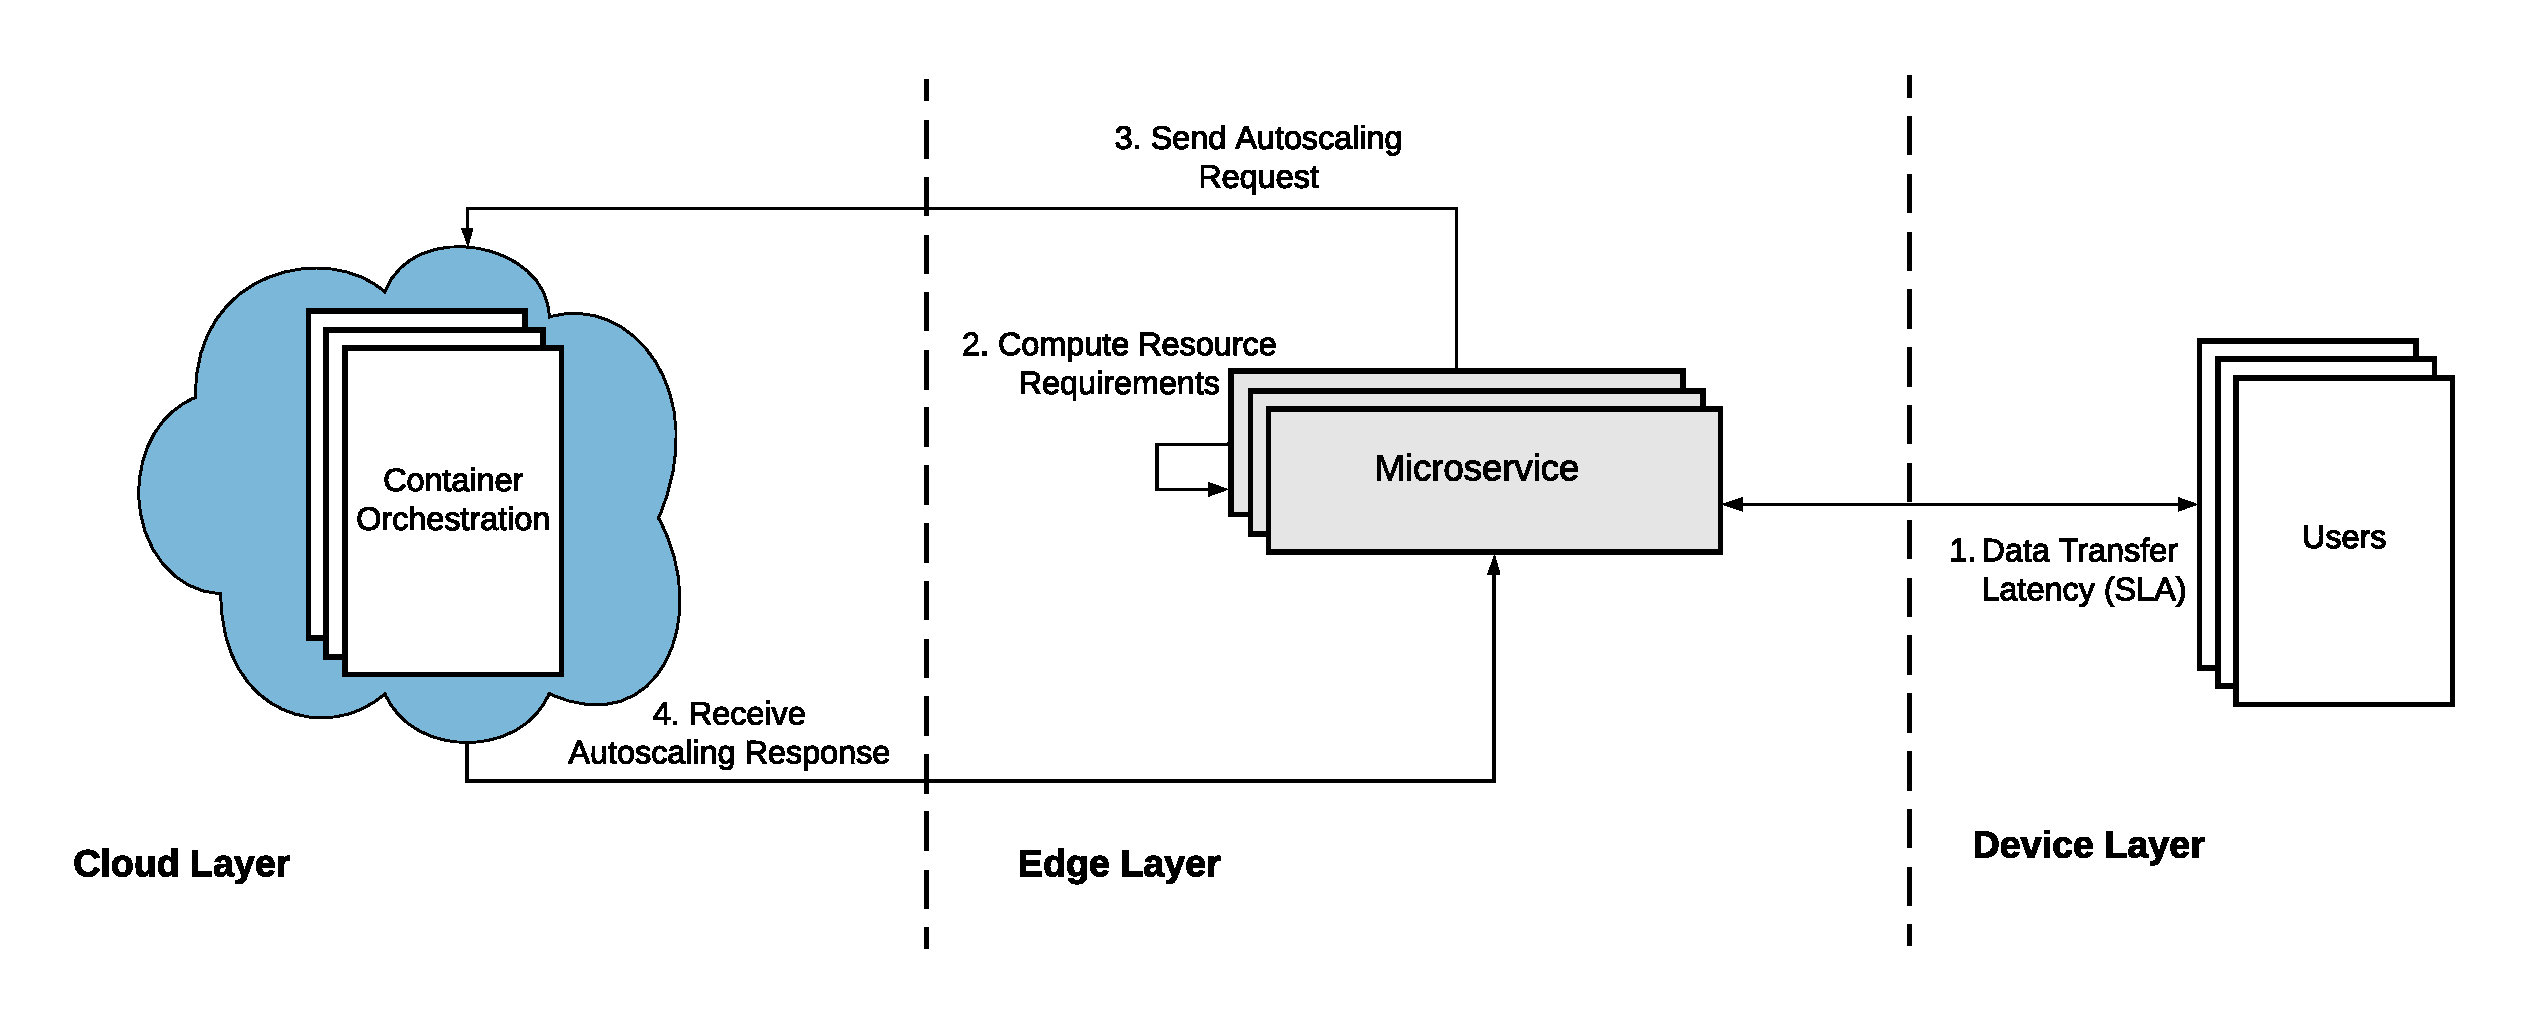
\includegraphics[width=0.8\linewidth]{Figures/Problem-Overview.pdf}
    \label{fig:autoscaling-problem-overview}
\end{figure}

The cloud layer has the most amount of resources allocated to it, as it is in charge of managing the entire network, and coordinating the resource allocation of the edge layer. However, the primary drawback is the distance between the user and the cloud layer which results in significant latency, making it unsuitable for serving real-time user requests. Thus only system critical applications such as the micro-service control plane are deployed on this plane. The edge layer has far fewer resources than the cloud layer, but its proximity to the users results in lower network latency, making it ideal for resources scaling. For this reason, the edge layer consists of the micro-service worker nodes. These nodes allocate resources dynamically according to user requirements through the process known as auto-scaling.\par

Figure \ref{fig:autoscaling-problem-overview} shows the auto-scaling process. The users in the device layer send requests and receive responses to the micro-service deployment in the edge layer. The time taken to receive this response is considered to be the SLA latency metric negotiated between the edge deployment provider and the customer. Using the number of requests being received by the user layer, the edge layer micro-service autoscaler computes the total resource requirements to serve the customer. Based on its findings, the edge layer requests the container orchestration in the cloud layer to either downscale or upscale its resources. The container orchestrator then computes the resource allocation location, and sends its response back to the edge layer.\par

%TC:ignore
\begin{table}
    \caption{Definition of Symbols}\label{tab:lstm-params}
    \centering
    \begin{tabular}{|l l|}
        \hline
        Symbol & Definition\\
        \hline
        $\mathcal{S}_{v}(t)$ & The value of the SLA metric at time $t$\\
        $\Delta$ & Maximum SLA metric threshold agreed by cloud provider and customer\\
        $\mathcal{C}_{t}$ & ``Cold start'' time taken to scale resource replicas\\
        $req_{RT}(t)$ & Round trip latency of user request to edge layer\\
        $\mathcal{K}_{t}$ & Constant latency present between edge and device layers\\
        $\mathcal{U}(t)$ & Latency of deployment with unitary resource replica\\
        $\mathcal{D}$ & Total resources in micro-service deployment\\
        $p_{i}$ & Resource pod $i$ of deployment $\mathcal{D}$ where $i = \{1, 2, .. N\}$\\
        \hline
    \end{tabular}
\end{table}
%TC:endignore

For real-time applications, the auto-scaling should adhere to SLA metric as much as possible, and try to minimize the number of violations. The SLA metric violation $\mathcal{S}_{v}(t)$ is defined as when it exceeds a certain threshold $\Delta$ agreed by both the cloud provider and the customer.
\begin{equation}
    \mathcal{S}_{v}(t) > \Delta
\end{equation}

The threshold $\Delta$ is typically split into three categories:
\begin{itemize}
    \item Flexible - This is typically the highest allowed violation threshold for the application. Flexible SLA metrics are used to gauge the availability of the deployment. Most IoT applications employ this threshold.
    \item Strict - This is the lowest allowed violation threshold in the application. This threshold is significantly challenging to maintain, and is used by extremely time-critical applications such as remote tools for surgery.
    \item Moderate - This threshold is a trade-off between flexible and strict SLA thresholds. This threshold is used by applications to ensure a real-time capability such as traffic light scheduling in railways.
\end{itemize}

The auto-scaling will thus use a resource metric to scale its resources up or down. The autoscaler will check to see if the micro-service metric exceeds the threshold for a certain time period, and if so, autoscale resources accordingly. A problem arises in the time it takes to scale these resources, however. This time to increase the number of resource replicas $\mathcal{R}$, known as cold start $\mathcal{C}(t)$ can be written as:

\begin{equation}
    \mathcal{C}(t) = \mathcal{R}_{download}(t) + \mathcal{R}_{deploy}(t) + \mathcal{R}_{register}(t)
\end{equation}

The replica download time is usually a one-time delay due to optimizations done on modern container orchestration software, and can be ignored for SLA latency calculations. Thus, we can reduce this equation to the following:

\begin{equation}
    \mathcal{C}(t) \approx \mathcal{R}_{deploy}(t) + \mathcal{R}_{register}(t)
\end{equation}


This time to deploy and register the replica to the container orchestration tool cannot be avoided. Furthermore, it can be shown that the number of SLA violations $\mathcal{V} \propto \mathcal{C}(t)$ due to the correlation between cold-start delay and the lack of available resources.\par

Thus, when computing the SLA violation for a latency metric, the SLA latency can be re-written as the sum of the cold-start time and the round-trip time taken for the request.

\begin{equation}
    \mathcal{S}_{v}(t) = \mathcal{C}(t) + req_{RT}(t)
\end{equation}


This round-trip time is the combined sum of the inherent delay present in the network layer, and the time taken for the edge application to process the request.

\begin{equation}
    req_{RT}(t) = 2 \times latency_{N/W} + latency_{app}
\end{equation}

The network delay can be reduced by investing in higher network bandwidths, but such improvements are out of scope of the project. Here we consider this latency to be a constant $\mathcal{K}$. Furthermore, $latency_{app}$ is inversely proportional to the available resources to the application. Using this information, $req_{RT}(t)$ is approximated as:

\begin{equation}
    req_{RT}(t) \approx \mathcal{K}(t) + \frac{\mathcal{U}(t)}{resources_{app}}
\end{equation}

Where $\mathcal{U}(t)$ is the app latency of a deployment with a unitary resource deployment. For horizontal pod autoscaling, the resources here are the number of pods in deployment $\mathcal{D}$ such that $\mathcal{D} = \sum_{i} p_{i}$, where $i$ represents the current number of deployed pods. These pods process the request. The final SLA equation can be re-written as follows:

\begin{equation}
    \mathcal{S}_{v}(t) = \mathcal{C}(t) + \frac{\mathcal{U}(t)}{\sum_{i} p_{i}} + \mathcal{K}(t)
\end{equation}

Thus, the primary aim of the proactive autoscaler is to significantly reduce or even eliminate the cold start, while the reactive autoscaler aims to increase the number of resources assigned to the deployment to minimize the application latency.\par

From the above equation, it is clear that as $\sum_{i} p_{i}$ approaches $\infty$, the value of $\frac{\mathcal{U}(t)}{\sum_{i} p_{i}}$ approaches 0. Thus, why not simply allocate the maximum number of pods to the deployment?\par

Most cloud providers allocate a cost $\mathcal{L}$ per each resource assignment to the deployment. If the maximum number of pods which can be deployed is $N$, the cost is calculated as follows.

\begin{equation}
    cost = \alpha \times \sum_{i} p_{i} \quad ;\,i \le N
\end{equation}

Where $\alpha$ is the unitary resource cost which may vary depending on the resource provider. Thus, simply scaling all resources to the maximum amount may result in significant and infeasibly high deployment costs. Thus the auto-scaling equation can be converted to an optimization problem. The objective of the autoscaler is to maximize resources in a way which minimizes both the latency, as well as the cost. Furthermore, the customer will have a maximum cost $\mathcal{L}$ which the deployment must not exceed. Determining whether or not the resource allocation of at least $\mathcal{D}$ without exceeding this cost $\mathcal{L}$ is possible, is akin to the famous Knapsack decision problem \cite{kellerer2004introduction}. This decision problem is NP-Complete, and as such no known algorithm can compute this auto-scaling decision in polynomial time \cite{martello1987algorithms}. Due to this drawback, most autoscalers rely on a reactive rule-based or proactive machine learning technique to compute a close approximation.\par

A problem arises, however, in the amount of time and resources it takes to train a proactive model. Not only is a significant amount of CPU and memory resources consumed in the training process, but a large time-series data set is also required to generate sufficient number of training windows, without which the model will provide erroneous results until such time as the model is adequately trained. While hybrid models help to mitigate the initial errors via the reactive auto-scaling component, the questions regarding the model complexity remained an open issue.\par

Another issue in proactive autoscalers is that not only does it predict increases in utilization before-hand, it also does so for the drop-off in utilization. This can lead to the edge deployment prematurely reducing its resources due to the drop-off forecast, causing several SLA violations due to low availability of resources. To offset this, several hybrid algorithms combine the readings of their reactive and proactive autoscalers, and autoscale according to the highest reading. While this approach works, such algorithms render the accurate resource drop-off predictions of the forecaster redundant, merely taking up precious computation space in the edge deployment.\par

In most proactive autoscalers, the forecaster attempts to perfectly model the time-series curve to assign resources. Even in the hybrid algorithms that have been proposed in chapter \ref{ch:background}, the proactive sections of the autoscalers are generally unmodified proactive forecasters bundled together with a reactive component. This strategy of attempting to perfectly forecasting the curve is what takes such large amounts of resources.\par

In the autoscaler proposed in this thesis, the autoscaler will not attempt to predict the exact resource workload. Instead, the time-series graph is heavily simplified using a noise filtering method, and then inputted to the machine learning model. Furthermore, the LSTM only attempts to forecast the exact times when resource requirements starts to increase. Every other requirement, such as the stable resource utilization, as well as the drop-off in non-peak time periods can be handled by the reactive autoscaler, thus heavily simplifying the forecaster architecture. The simplified forecaster has an additional benefit in not requiring incredibly lengthy amounts of time-series data to be stored for it to make accurate predictions, thus this data can also be kept in the edge layer. This makes the autoscaler extremely lightweight and responsive, and thus capable of being deployed in an edge environment.\par

\section{Proposed Hybrid Autoscaler}
\label{sec:ch3-hybrid-autoscale-overview} 

\begin{figure}[htb]
    \centering
    \caption{Proposed hybrid architecture overview}
    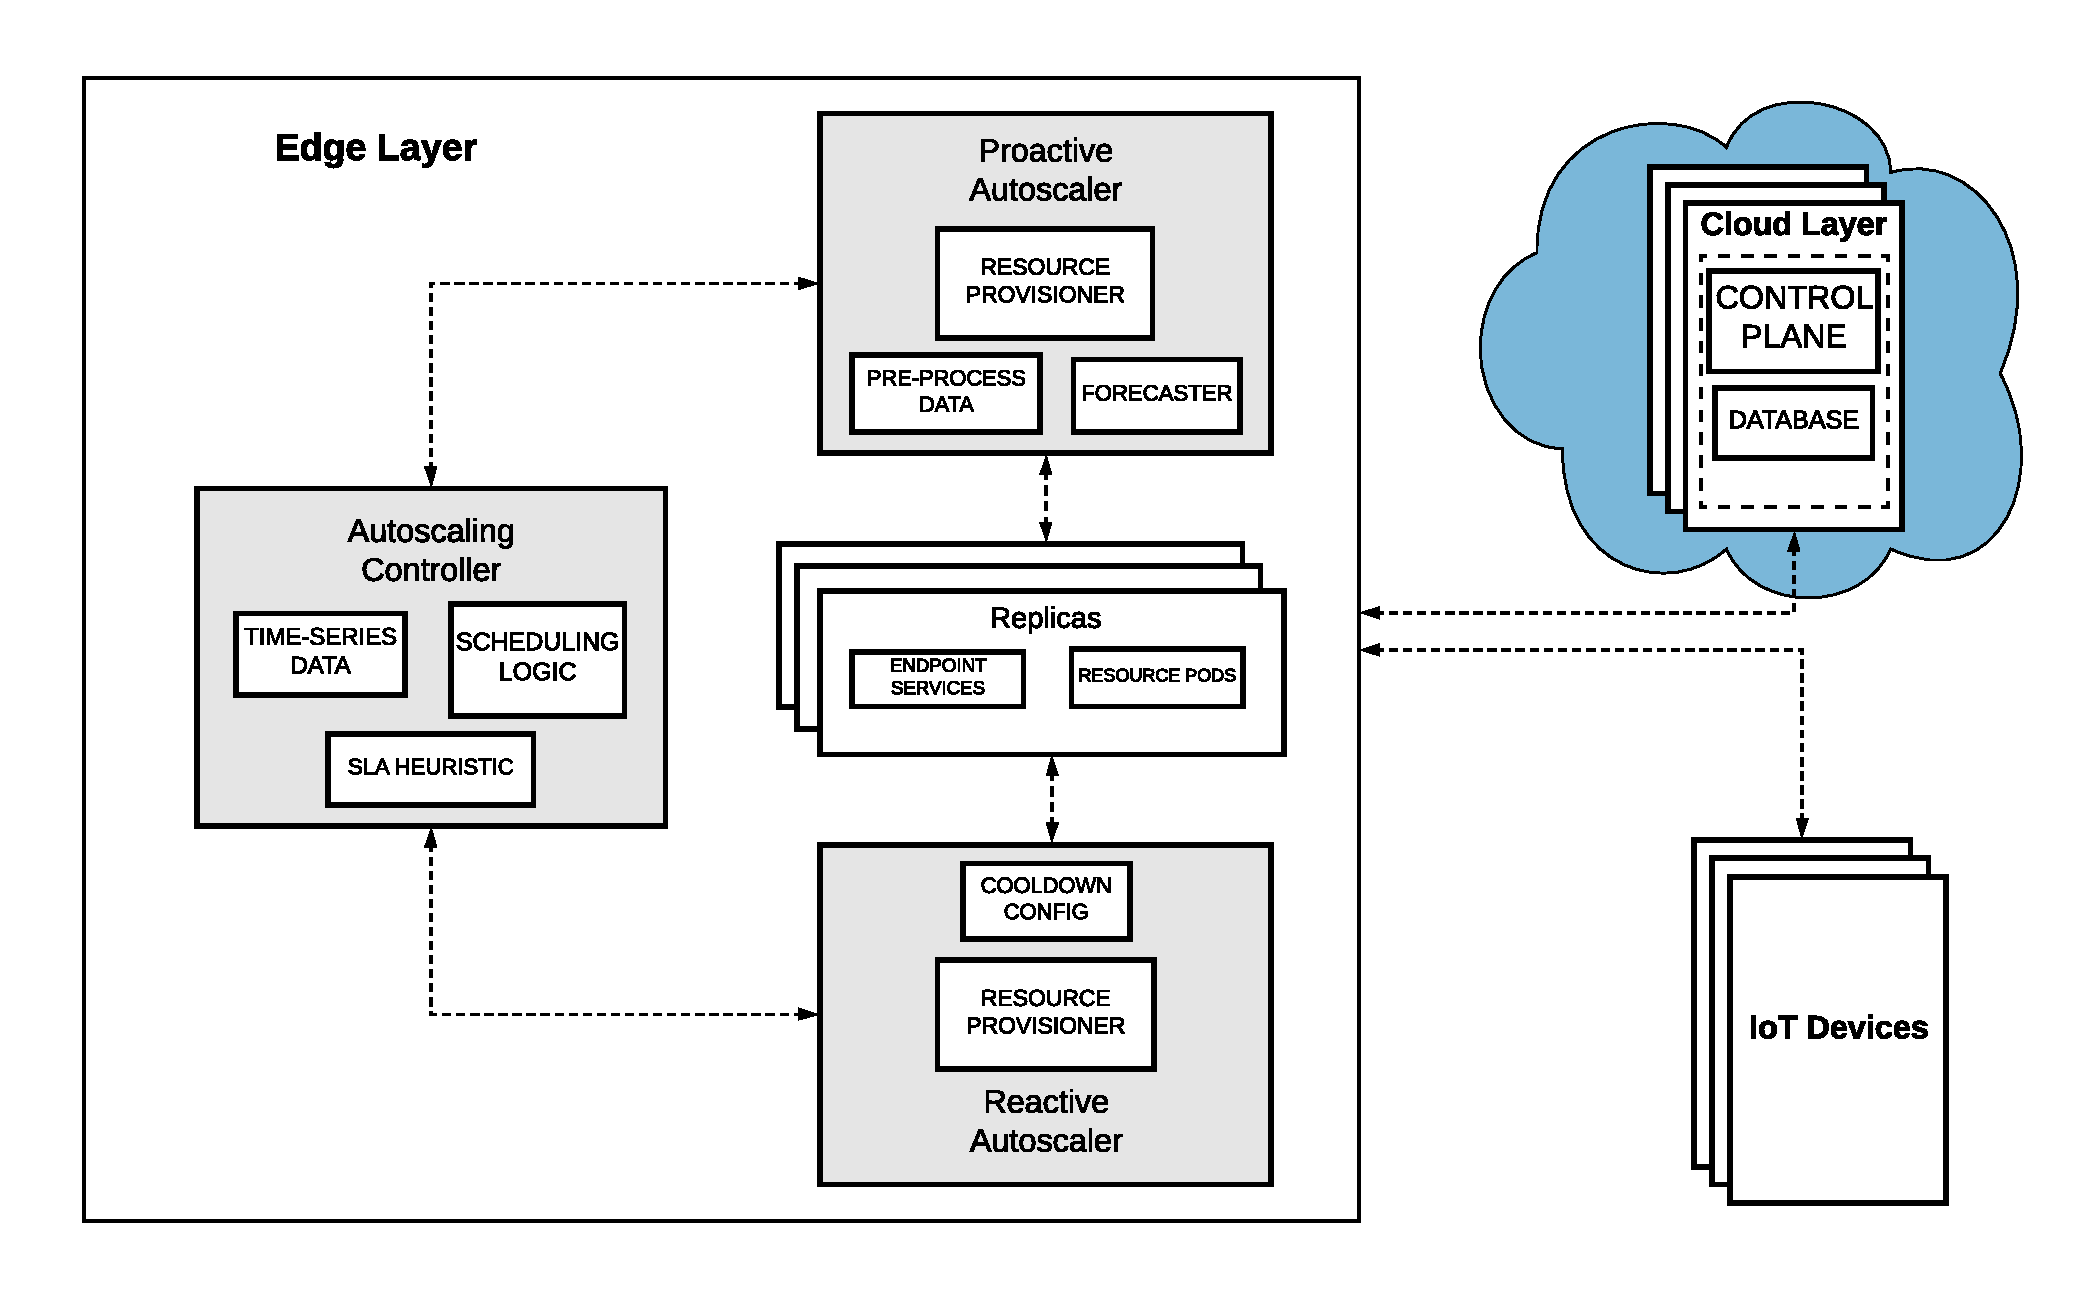
\includegraphics[width=1.0\linewidth]{Figures/Hybrid-Architecture-Overview.pdf}
    \label{fig:hybrid-arch-overview}
\end{figure}

An overview of the hybrid autoscaler architecture is shown in figure \ref{fig:hybrid-arch-overview}. The edge node consists of three main sections. The first is the reactive autoscaling subsystem, which has the resource provisioner, and the configuration which dictates the cool-down logic for scaling up and down. As Zhang et al. \cite{zhang2019quantifying} demonstrated, the microservice system stability is directly related to the careful selection of cooldown parameters. Thus, these must be available to the user in a configuration setting.\par

\suhrid{TODO: Make sure to discuss the proactive autoscaler in detail in Ch3 using the notes written in Ch2 \cmark}
The second subsystem is the proactive autoscaler. From a high-level perspective there are three main components. The resource provisioner is similar to that of the reactive autoscaler, however it also consists of a forecaster using machine learning techniques, and a data pre-processing algorithm. This algorithm removes any noise present in the time series data, and smoothens the graph, making it easier for the forecaster to make predictions in a low-cost manner. A detailed explanation of the forecaster logic itself will be discussed in chapter \ref{ch:experimental-setup}.\par

Finally, the auto-scaling daemon controls which auto-scaling logic will be applied to the replicas, and also keeps a track of any SLA violations. It also hosts the time-series metric data, and has a feedback loop with the proactive autoscaler. If it detects any SLA violations caused after autoscaling during a configured time window, it automatically adjusts the hyper-parameters of the proactive forecaster in an attempt to predict the time-series in a more accurate manner during the next training iteration. Correspondingly, a lack of SLA violations during a specific time period reverts the autoscaler parameters to attempt to streamline the training process further. Such a heuristic method allows for the freeing up of the complex hyper-parameter tuning process seen in most proactive models. This is a key part of the architecture which is essential in answering one of the research questions outlined in the thesis.\par

\suhrid{In methodology, detail the reactive and proactive portions - detail only the algorithm pseudo-code \cmark}

\subsection{Architecture Overview}
\label{subsec:ch3-hybrid-arch}

At a high-level, the default Kubernetes horizontal pod autoscaler operates on the ratio between the current and desired metric values, which can be written as:

\begin{equation}
    replicas_{desired} = \lceil replicas_{current} \times \frac{metric_{current}}{metric_{desired}}\rceil
\end{equation}

For example, for a given deployment with current replica count as 1, if the desired metric value is 50 resource units, the current value is 100, then the number of desired replicas will be $\lceil 1 \times \frac{100}{50}\rceil = 2$. There are three other important parameters which are key to controlling the process of horizontal pod scaling, namely ``tolerance'', ``scale up cooldown'', and ``scaledown cooldown''.\par

The tolerance is a constant which informs the Kubernetes autoscaler when to skip calculating new replicas. The tolerance ratio, can be calculated as:

\begin{equation}
    \label{eqn:tolerance}
    tolerance = \abs{ \frac{metric_{desired} - metric_{current}}{metric_{desired}} }
\end{equation}

For example, if the current metric is 60, and the desired metric is 50, the tolerance is calculated as $ tolerance = \abs{ \frac{60 - 50}{60}} = 0.167$. By default, if the tolerance value is below 0.1, autoscaling is skipped for that control loop, however this can be configured by the user.\par

The scale up and scale down cooldowns control how quickly autoscaling occurs. The default approach which is set by Kubernetes can be concisely stated as ``Scale up as quickly as possible, while scale down very gradually''. Therefore, the default scale up cooldown is set to 0 seconds, meaning that the moment the desired replica value increases, the autoscaling will be initiated. However, the default cooldown is set to 300 seconds, meaning that if the desired replica value is decreased, it must remain decreased for 300 seconds (or 20 control loops) before the resources are scaled down.\par

A cooldown value which is too low would cause a repetitive upscaling and downscaling of the resources, leading to a significant stress on the system as well as a wastage of resources. Meanwhile, a large value would render the autoscaler unable to assign resources quickly enough to ensure SLA latency compliance. Thus, for the proposed autoscaler, a moderate cooldown value was chosen to ensure best system stabilty and SLA compliance. This cooldown configuration would be applied to both the proactive and reactive auto-scaling sub-components.\par

For auto-scaling proactively, a custom metric $metric_{forecast}$ is used, which defines the future CPU workload expected to be exerted on the social media application $\mathcal{T}$ seconds in the future, where $\mathcal{T}$ can be configured by the user. This $metric_{forecast}$ value will be sent to the auto-scaling daemon by the proactive autoscaler.\par

The autoscaler daemon consists of a scheduling logic controller which handles how to switch between proactive and reactive auto-scaling. Algorithm \ref{alg:scheduling-logic-daemon} explains how the hybrid scheduling logic determines which auto-scaling subsystem to employ. The hybrid scheduler takes four inputs, namely the $replicas_{current}$, $metric_{current}$, $metric_{desired}$, and $metric_{forecast}$ variables discussed above. It outputs one value, the $replicas_{desired}$.\par

The autoscaler computes two replica values, one for the proactive forecaster which determines the replicas after $\mathcal{T}$ seconds, and one for the reactive forecaster, which determines the current resource requirements. If it is found that the future requirements are higher than the current resource utilization, then the hybrid scheduler outputs the forecaster replica count as the desired replicas. Otherwise, the hybrid scheduler determines that the utilization is either stabilizing or about to decline. Due to this, it makes a decision that the reactive replica count is the desired number. The hybrid scheduler then sends this value to the container orchestration controller plane to autoscale the replicas accordingly using either the reactive or proactive sub-system's resource provisioner.\par

%TC:ignore
\begin{algorithm}
    \caption{Scheduling logic of the autoscaler daemon}
    \label{alg:scheduling-logic-daemon}
    \textbf{Input}: $replicas_{current},\, metric_{current},\, metric_{desired},\, metric_{forecast}$\\
    \textbf{Output}: $replicas_{desired}$
    \begin{algorithmic}
        \State $replicas_{forecast} \gets \lceil replicas_{current} \times \frac{metric_{forecast}}{metric_{desired}}\rceil$
        \State $replicas_{reactive} \gets \lceil replicas_{current} \times \frac{metric_{current}}{metric_{desired}}\rceil$
        \If{$replicas_{forecast} > replicas_{reactive}$}
            \State $replicas_{desired} \gets replicas_{forecast}$
        \Else
            \State $replicas_{desired} \gets replicas_{reactive}$
        \EndIf
        \State \Return $replicas_{desired}$
    \end{algorithmic}
\end{algorithm}
%TC:endignore

The reactive autoscaler subsystem is responsible for determining whether or not auto-scaling should proceed based on the given configuration. The reactive algorithm is built on top of the default horizontal pod autoscaler deployed by the container orchestration platform. The autoscaler is modified in such a way that it has its cooldown parameters are set to a moderate value to ensure adaptability to SLA-constrained scenarios, while also maintaining system stability. The workflow is shown below in algorithm \ref{alg:reactive-algo}. The algorithm takes the desired and current metrics as input, as well as the desired metrics, and outputs the decision to autoscale or not. It does this by computing the $tolerance$ value as shown in equation \ref{eqn:tolerance}. If this tolerance is above the configured threshold, the autoscaler will be modify the replicas, otherwise it will ignore the current auto-scaling request.\par

%TC:ignore
\begin{algorithm}
    \caption{Reactive autoscaler subsystem workflow}
    \label{alg:reactive-algo}
    \textbf{Input}: $metric_{current},\, metric_{desired}$\\
    \textbf{Output}: $autoscale$
    \begin{algorithmic}
        \State $tolerance \gets \abs{ \frac{metric_{desired} - metric_{current}}{metric_{desired}} }$
        \If{$tolerance > \gamma$}
            \State $autoscale \gets Yes$
        \Else
            \State $autoscale \gets No$
        \EndIf
        \State \Return $autoscale$
    \end{algorithmic}
\end{algorithm}
%TC:endignore

The forecaster portion of the autoscaler is used to generate this $metric_{forecast}$ value. Several time series forecaster algorithms exist, with the two prominent ones being the more modern deep learning algorithm LSTM, and the traditional deep learning algorithm ARIMA. Siami-Namini et al. \cite{siami2018comparison} demonstrated that LSTM implementations outperformed ARIMA, reducing error rates by over 80\%. Furthermore, they were able to demonstrate that the number of deep learning ``epochs'', or the total amount of training time required for LSTM did not need to be set to a high value. In fact, setting an significantly higher value than required was shown to degrade performance due to over-fitting. The authors posited that LSTM worked so well due to the ``rolling updates'' being performed on the model. The LSTM weights are only set once when the forecaster is deployed, after which they are always updated on every call of the training algorithm, meaning there is a continuous improvement to the prediction results.\par

\begin{figure}[htb]
    \centering
    \caption{Pre-processing of data, courtesy of Christopher Boucher \cite{comsolcurvefitting}}
    \label{fig:data-pre-process}
    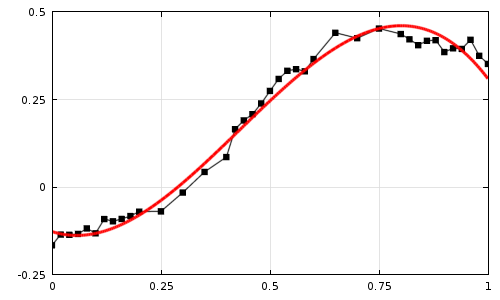
\includegraphics[width=0.6\linewidth]{Figures/Data-Pre-Processing.png}
\end{figure}

To speed up the forecast process even further and reduce the resource and time requirements, the time-series data can be pre-processed to smoothen it. Doing so makes it easier for the deep learning model to extract patterns, and reduces the training and validation loss. Figure \ref{fig:data-pre-process} shows a graph containing raw input (shown in black), and a smoothened data curve (shown in red). While the red curve contains all the requisite information of the data (such as slope of the curve, maximum and minimum value, etc.), it removes the noise, reducing the overall loss, and reducing the length of the lookback LSTM needs to perform to accurately predict future data.\par

Based on the investigations above, it was determined that LSTM time-series forecasters would be ideally suited for a proactive autoscaler designed for edge computing. Algorithm \ref{alg:proactive-forecast-alg} shows the implementation of such a forecaster. As input, the algorithm takes the variable $lookback$, which is the number of data points it should use as a window to train, $forecast$, which is the number of data points to predict, the training time $epochs$, and the $learning\_rate$, which determines the step size per each training iteration moving towards the minimum loss value. The algorithm outputs the $result$, which is an array of size $forecast$ which contains all the predicted values. The algorithm implements a control loop every $\mathcal{P}$ seconds, where it requests the latest time series data from the autoscaler daemon. It then pre-processes this data to remove the noise as shown above, and performs one iteration of training using the configured parameters. It then computes the validation loss when doing so, and accepts this model as the ideal one if it has lower validation loss than the previous iteration, otherwise rejecting the model and using the older one instead. Finally, the model predicts the future forecasts and returns them to the autoscaler daemon for later use.\par

%TC:ignore
\begin{algorithm}
    \caption{Proactive forecaster algorithm}
    \label{alg:proactive-forecast-alg}
    \textbf{Input}: $lookback \geq 0, forecast \geq 0, 0 \leq epochs \leq 100, 0 \leq learning\_rate \leq 1$\\
    \textbf{Output}: $result$
    \begin{algorithmic}
        \State $lstm\_model \gets lstm.initialize()$
        \State $result \gets \varnothing$
        \While{$true$}
            \State $time\_series \gets get\_latest\_data()$
            \State $lstm\_input \gets get\_input(time\_series\_data, lookback)$
            \State $lstm\_input \gets preprocess\_data(lstm\_input)$
            \State $new\_model \gets train(lstm\_input, epochs, learning\_rate)$
            \If{$validation\_loss(new\_model) < validation\_loss(lstm\_model)$}
                \State $lstm\_model \gets new\_model$
            \EndIf
            \State $result \gets predict(lstm\_model, lstm\_input, forecast)$
            \State \Call{wait}{$\mathcal{P}$}
        \EndWhile
    \end{algorithmic}
\end{algorithm}
%TC:endignore

Finally, the other two sub-systems of the autoscaler daemon architecture help the proactive forecaster increase its prediction accuracy. It consists of the decision making and feedback loop of the proactive forecaster, and the storage of time-series data of the edge node.\par

%TC:ignore
\begin{algorithm}
    \caption{Get predicted CPU value at time $\mathcal{T}$}
    \label{alg:get-forecast-value}
    \textbf{Input}: $\mathcal{T} > 0$\\
    \textbf{Output}: $metric_{forecast}$
    \begin{algorithmic}
        \State $time\_series \gets [ \vartheta_1, \vartheta_2 .. \vartheta_n ]$
        \State $current\_time \gets get\_time()$
        \State $threshold \gets \omega$
        \State $metric_{forecast} \gets 0$
        \State $closest\_index \gets time\_series.get\_index(\mathcal{T}, current\_time, threshold)$
        \If{$time\_series[closest\_index] exists$}
            \State $metric_{forecast} \gets time\_series[closest\_index]$
        \EndIf
        \State \Return $metric_{forecast}$
    \end{algorithmic}
\end{algorithm}
%TC:endignore

The time series data not only includes the historical resource data, but also the predicted data created by the forecaster. The daemon periodically scrapes the windowed data stored in the cloud database to keep a form of cached time-series workload. It combines this workload with the future workload generated by the forecaster. The proactive autoscaler can then request the future workload for a specified time $\mathcal{T}$, and the daemon either sends back the forecasted value, or $0$ if it does not exist. Algorithm \ref{alg:get-forecast-value} depicts this process. The algorithm computes the nearest index in the time-series forecasted data containing the value. The nearest index is limited to a certain threshold, so that the time difference between what is requested, and what is computed is not too large since that would cause an error in the autoscaling. If this index exists in the data, the resource value is returned to the autoscaling daemon to be served to the proactive autoscaler, otherwise the default value of $0$ is sent.

%TC:ignore
\begin{algorithm}
    \caption{SLA-based feedback loop for proactive forecaster}
    \label{alg:sla-heuristic-feedback}
    \textbf{Input}: $SLA\_violation\_count,\,learning\_rate,\,batch\_size,\,epochs$\\
    \textbf{Output}: $hyperparameters_{modified}$
    \begin{algorithmic}
        \State $initial\_rate \gets learning\_rate$
        \State $initial\_batch \gets batch\_size$
        \State $initial\_epochs \gets epochs$
        \If{$SLA\_violation\_count$ > 0}
            \State $batch\_size \gets MAX(batch\_size + \alpha, \mathcal{A})$
            \State $learning\_rate \gets MIN(learning\_rate - \beta, \mathcal{B})$
            \State $epochs \gets MIN(epochs - \lambda, \mathcal{L})$
        \Else
            \State $epochs \gets initial\_epochs$
            \State $learning\_rate \gets initial\_rate$
            \State $batch\_size \gets initial\_batch$
        \EndIf
        \State $hyperparameters_{modified} \gets (learning\_rate, batch\_size, epochs)$
        \State \Return $hyperparameters_{modified}$
    \end{algorithmic}
\end{algorithm}
%TC:endignore

The final component of the autoscaler daemon is the SLA-based feedback for the proactive forecaster. The autoscaler constantly checks for SLA-violations in the edge deployment using a control loop. Typically, the SLA checks are done for a sufficiently lengthy period of time such as one day. If an SLA violation is found, it is concluded that the application was unable to autoscale quickly enough to avoid the cold start problem. This could be due to a number of causes, such as insufficient training data, or the LSTM hyper-parameters being too conservative. To temporarily boost learning, the daemon then decreases the learning rate to increase the probability of the model escaping from the local minima to find the global one, increases the batch size to reduce under-fitting, and increases the number of epochs to reduce loss. All these parameters have a threshold, as increasing or decreasing certain parameters by a large amount may lead to issues such as over-fitting or infeasibly lengthy training times. Finally, if the feedback control loop discovers that no SLA-violations occurred during the time-period, it concludes that the LSTM has sufficiently learned the primary characteristics of the time-series. As discussed by Siami-Namini et al. \cite{siami2018comparison}, the ``rolling-updates'' feature of LSTM allows the autoscaler to safely reset the hyper-parameters of the model, while preserving the learning and weights of the previous rounds of training. Algorithm \ref{alg:sla-heuristic-feedback} shows how the heuristic feedback is set up. The algorithm takes the three hyper-parameters of the LSTM, namely $learning\_rate$, $batch\_size$, and $epochs$, along with the $sla\_violation\_count$ which stores the number of SLA violations which occurred during a specified time window. Using these parameters, the algorithm computes the new LSTM hyper-parameters and outputs them to the proactive forecaster to use in the next training cycle.\par

\subsection{Space Time Complexity}
\label{subsec:ch3-space-time-comp}

Assuming the hybrid autoscaler $\mathcal{H}$ takes a time-series data of length $\mathcal{N}$, it stores this data in an array data structure. The rest of the inputs are single variables. Thus the space complexity can be easily computed for this information. The variables each have a space complexity of $O(1)$. Meanwhile, the time-series array has a complexity of $\mathcal{O}(N)$. Thus, the space complexity can be written as the sum of the two values, and simplified.

\[Complexity_{space}(\mathcal{H}) = \mathcal{O}(N) + \mathcal{O}(1)\]
\begin{equation}
    \Rightarrow Complexity_{space}(\mathcal{H}) = \mathcal{O}(N)
\end{equation}

The time complexity is a more complex calculation. The complexities of the reactive autoscaler, proactive autoscaler, and autoscaler daemon need to be computed. The autoscaler daemon only stores the time-series array, and computes the new hyper-parameters in algorithm \ref{alg:sla-heuristic-feedback}. Both of these operations can be completed in constant time, thus the time complexity for the daemon is as follows:

\begin{equation}
    Complexity_{time}(daemon) = \mathcal{O}(1)
\end{equation}

Similarly, the reactive autoscaler only computes the tolerance value, which is also a constant operation independent of data size, thus the time complexity can be written as:

\begin{equation}
    Complexity_{time}(reactive) = \mathcal{O}(1)
\end{equation}

For the proactive autoscaler, the forecaster internally computes matrix multiplications, such as of the various LSTM weights and vectors. For example, take the equation \ref{eqn:input-gate}. In the equation, we assume the dimension of the variables as follows:

\begin{itemize}
    \item $W_{i} \in \R^{m \times n}$
    \item $x_{t} \in \R^{n}$
    \item $b_{i} \in \R^{m}$
    \item $h_{t-1} \in \R^{m}$
\end{itemize}

Using these values, the time complexity of each of the individual multiplicative and additive operations can be computed.

\begin{itemize}
    \item $Complexity_{time}(W_{i} \cdot x_{t}) = \mathcal{O}(mn)$
    \item $Complexity_{time}(W_{i} \cdot h_{t-1}) = \mathcal{O}(mn)$
    \item $Complexity_{time}(W_{i} \cdot [x_{t}, h_{t-1}]) = \mathcal{O}(mn + mn + m)$
\end{itemize}

Therefore the complexity of the proactive component can be written as:

\[Complexity_{time}(proactive) = \mathcal{O}(mn + mn + m)\]
\[\Rightarrow Complexity_{time}(proactive) = \mathcal{O}(2mn + m)\]
\[\Rightarrow Complexity_{time}(proactive) = \mathcal{O}(m \times n)\]
\begin{equation}
    \Rightarrow Complexity_{time}(proactive) = \mathcal{O}(N^2)
\end{equation}

This 

Combining the time complexities of all three hybrid components, the final complexity for the hybrid autoscaler $\mathcal{H}$ can be re-written as:

\[Complexity_{time}(\mathcal{H}) = \mathcal{O}(1) +  \mathcal{O}(1) + \mathcal{O}(N^2)\]

\begin{equation}
    \label{eqn:hybrid-time-complexity}
    \Rightarrow Complexity_{time}(\mathcal{H}) = \mathcal{O}(N^2)
\end{equation}

From the results in equation \ref{eqn:hybrid-time-complexity}, it is clear that the hybrid algorithm performs extremely well in a polynomial time complexity. Even though it is shown that no mathematically certain decision can be computed in a polynomial time due to the NP-Completeness of the problem statement, the hybrid algorithm provides an alternative which is able to approximate with high accuracy an auto-scaling decision in polynomial time.
\clearpage

\def\chaptertitle{System Implementation}

\lhead{\emph{\chaptertitle}}

\chapter{\chaptertitle}
\label{ch:experimental-setup}

Based on the previous high-level overview of the architectures and algorithms involved, in this chapter, we will first discuss the micro-service application architecture used to test the algorithm, along with its features in section \ref{sec:ch4-microservice-overview}. Based on this, section \ref{sec:ch4-data-generation} will give an explanation of the workload generator bundled along with the micro-service deployment, and how that is used to generate the time-series workload typically seen in edge architectures. Finally, we will discuss the technical configurations of the hybrid autoscaler itself in section \ref{sec:ch4-hybrid-auto-arch}. This will involve how the workload information is communicated between cloud and edge layers, how the autoscaler parameters for both reactive and proactive subsystems are configured, and how the forecaster is configured to use the time-series data to generate forecasted values for a sufficiently large time-period.

\section{Microservice Overview}
\label{sec:ch4-microservice-overview}

DeathStarBench \footnote{\url{https://github.com/delimitrou/DeathStarBench/tree/master/socialNetwork}}, a social media micro-service developed by Y. Gan et al. \cite{gan2019open} is ideal for benchmarking SLA-compliance, and was thus deployed on Kubernetes. The application mimics a large-scale social network application and supports common actions such as registering and login for user credentials, creating user posts on their timeline, reading other user timelines, receiving follower recommendations, following and unfollowing of other users, and searching for users or posts. Figure \ref{fig:social-network-arch} shows the architecture of the micro-service.\par

\begin{figure}[htb]
    \centering
    \caption{DeathStarBench Social-Network Architecture, courtesy Y. Gan et al. \cite{gan2019open}}
    \label{fig:social-network-arch}
    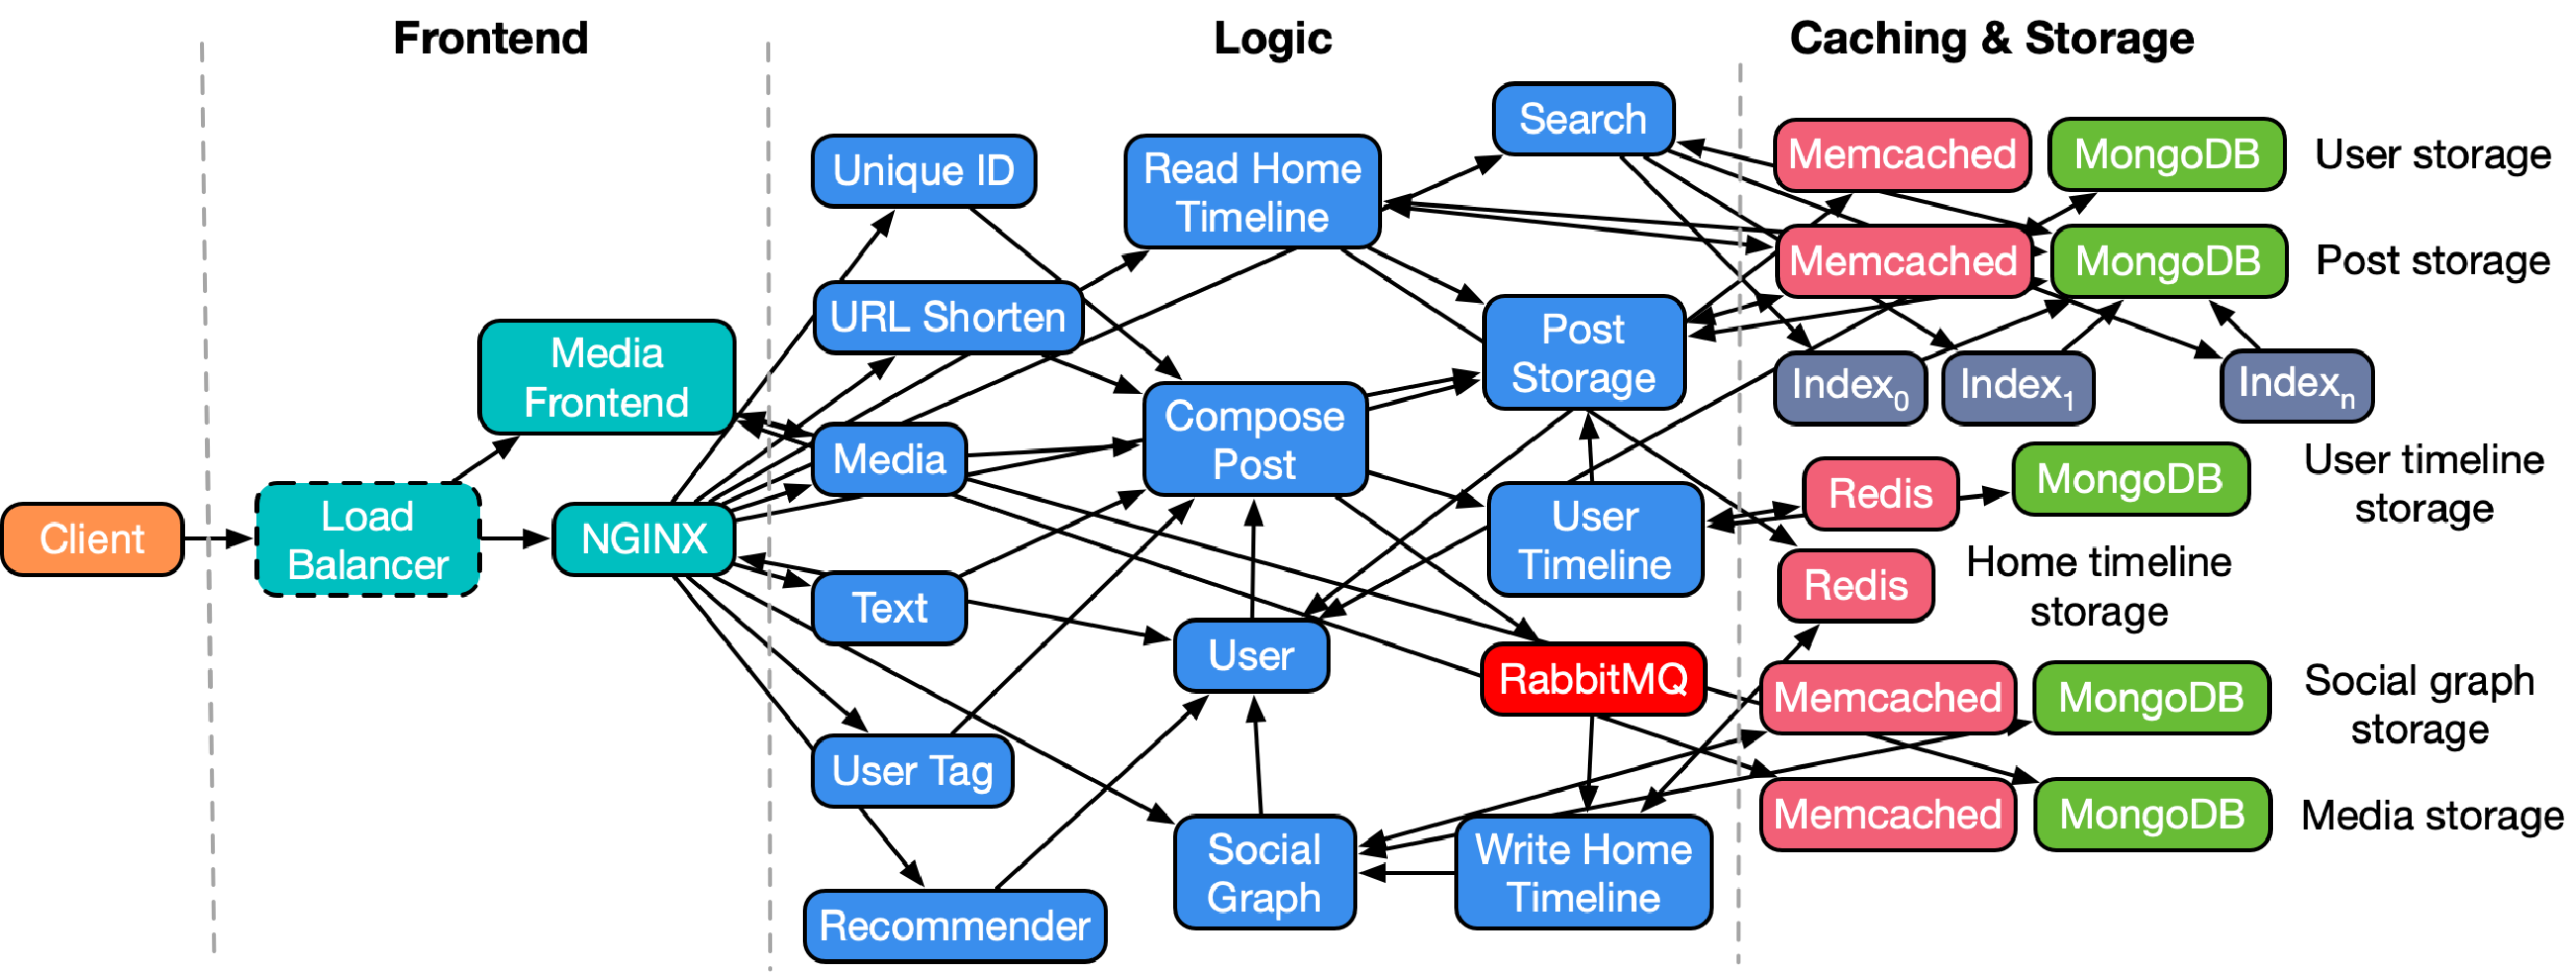
\includegraphics[width=1.0\linewidth]{Figures/Social-Network-Architecture.pdf}
\end{figure}

The end-to-end service implementation depicts a social network with a broadcast style approach. The user or client sends requests using HTTP to the front-end layer. These requests are processed using a load balancer implemented using an open-source deployment known as NGINX \footnote{\url{https://nginx.org/en/}}. NGINX then specifies the web server that has been selected, and communicates with the micro-services in the logic layer, which are responsible for composing and displaying the user and timeline posts. The logic layer also consists of micro-services for serving advertisements, search engines, and other capabilities commonly found in large scale applications. The search and advertisement engines are machine learning plugins capable of serving recommendations based on user interactions. The logic layer is capable of handling posts containing text, links, and media. Users can also mark other user's posts as favourites, re-post them, and reply to them privately or publicly. Users can also follow, unfollow, or block others. All these interaction results are stored in the storage layer, which uses memcached for caching results, and MongoDB for storing user profiles, posts, media, and recommendations in a persistent manner.

Users can sign in to the application website by connecting to the user interface deployment, which can be assigned a DNS address. For simplicity, in this experiment the Kubernetes node IP address was exposed through the deployment, along with the social media application port. For example, an API request for reading user timelines will look as follows:\par

\begin{lstlisting}[
  caption={Social network API call template},
  captionpos=t,
  label={lst:social-network-api-template},
]
http://<node-IP>:<app-port>/wrk2-api/user-timeline/read
\end{lstlisting}

\section{Data Generation}
\label{sec:ch4-data-generation}

The social media deployment also comes with an HTTP workload generator, which
is leveraged to create a realistic simulation of a typical day of workload for the microservice application. The generator, known as ``wrk2'', is an open-loop load generator. HTTP requests are sent out according to the user configuration, regardless of whether or not the responses of the previous requests have been received. This avoids issues such as queuing delays in the server, helping to maintain an even load throughout the generation process which aids in benchmarking. The workload generator supports a variety of load generation use-cases, as well as different APIs. For example, a POST request with a total load generation of 8 requests per second, using 2 parallel threads, with 5 open HTTP connections, and for a duration of 30 seconds looks as follows:\par

\begin{lstlisting}[
  caption={Workload generation example},
  captionpos=t,
  label={lst:workload-gen-example},
  language=bash
]
$ wrk2 -t2 -c5 -d30 -R8 http://<node-IP>:<app-port>/wrk2-api/post/compose
\end{lstlisting}



A typical IoT application in the edge has a semi-predictable workload pattern. In this experiment, it is assumed that the workload peaks in the morning and evening, while seeing moderate usage during the afternoon. The workload is lowest at night. The workload simulator was modified to introduce an element of randomness to mimic realistic weekly workloads, which can vary on occasions such as weekends and public holidays.\par

To achieve this, an IoT workload algorithm was created for leveraging the wrk2 generator to achieve this time-series. This is explained in algorithm \ref{alg:work-gen}. A constant light workload is set for night time consisting of six hours between 12:00am and 06:00 am, while different workloads for the eighteen different day time hours are set, with peaks set in the morning and evening, and dips in the afternoon. The algorithm also contains a small random ``offset'' variable to depict the randomness inherent in the workload. This is depicted using the function $\mathcal{U}$, where $\mathcal{U}(0,1)$ returns a random number between 0 and 1. This workload is then executed using the wrk2 generator to apply the HTTP load on the microservice.

%TC:ignore
\begin{algorithm}
    \caption{IoT workload generation algorithm}
    \label{alg:work-gen}
    \begin{algorithmic}
        \State $offset \gets \alpha$
        \State $night\_workload \gets \omega$
        \State $day\_workload \gets [ \delta_1, \delta_2, ... , \delta_{18}]$
        \While{True}
            \For {i $\leftarrow$ 0 ... 6}
                \State $result \gets generate(night\_workload + \mathcal{U}(-offset,offset)$
            \EndFor
            \For {i $\leftarrow$ 0 ... 18}
                \State $result \gets generate(day\_workload[i] + \mathcal{U}(-offset,offset)$
            \EndFor
        \EndWhile
    \end{algorithmic}
\end{algorithm}
%TC:endignore

\section{Hybrid Autoscaler Configuration}
\label{sec:ch4-hybrid-auto-arch}

\suhrid{Move all algorithm pseudo-code to ch3, move lstm justification to ch3, all code implementation should remain here \cmark}

In this section, the configuration parameters of the proposed hybrid autoscaler will be discussed. First, a brief background will be provided of how the social network application is connected to Kubernetes, so that it can send default and custom metrics such as application CPU usage and latency respectively. These custom metrics will then be discussed further, and how they are integrated for use in the horizontal pod autoscaler.\par

With this background, a further discussion of the reactive subcomponent of the hybrid autoscaler is conducted, explaining its parameters and how it connects to the custom metrics API. The details of the proactive autoscaler are then discussed. This includes the architecture of the LSTM, default hyper-parameters, and the lookback and forecasting window. Finally, the autoscaler heuristic feedback will be discussed, including the exact parameters it modifies when it discovers an SLA violation.\par

\subsection{Custom Metrics Export To Kubernetes}
\label{subsec:metrics-export}

The social media application comes bundled with Jaeger \footnote{\url{https://www.jaegertracing.io/}} deployment. Jaeger is an open-source distributed tracing platform, capable of tracking several application metrics of each network request and per-microservice request, and stores them in a centralized database. One such metric is the details of API latency for the application. The latency information is extremely detailed, and is broken down per each deployment in the social media architecture as defined by Figure \ref{fig:social-network-arch}. Alongside the latency breakdown, Jaeger can automatically generate graphs of the Kubernetes deployments which are utilized by API calls. This is particularly useful for identifying deployment bottlenecks which are prime targets for autoscaling.\par

Before this latency information can be useful in the autoscaling solution, it must be imported to Kubernetes in a readable format. This was achieved through the use of a tool called Prometheus. Prometheus \footnote{\url{https://prometheus.io/docs/introduction/overview/}} is an open-source deployment used for monitoring applications. Prometheus consists of a multi-dimensional data model for storing time-series data through key/value pairs, a custom built querying language known as PromQL, which is used to leverage and search through this data model, and a graphing and dashboard user interface to aid in visualization. Due to the heavy nature of the deployment, Prometheus must be deployed on the cloud layer.\par

%TC:ignore
\begin{lstlisting}[
  caption={Jaeger-Scraper server},
  captionpos=t,
  label={lst:jaeger-scraper},
  float=ht
]
const avg_counter = new Gauge({
        name: 'wrk2_avg_api_latency',
        help: 'Jaeger average post API latency (ms)'
});

get('/metrics', async (req, res) => {
    let url = process.env.JAEGER_URL;
    const data = await axios.get(url);
    let avg_duration = 0;

    let durations = data.map(components => {
        let duration = components.duration;
        return duration;
    });

    avg_duration = durations.reduce( (a,b) => a+b ) / durations.length;
    avg_counter.set(avg_duration);

    result.set('Content-Type', avg_counter);
});
\end{lstlisting}
%TC:endignore

To facilitate the export of Jaeger metrics to Prometheus, a custom deployment was created which scrapes these metrics at a given time interval, and pushes it to Prometheus. The deployment, which was named ``Jaeger-Scraper'', was a JavaScript express server set up on Kubernetes using Docker, and the server code was as shown in listing \ref{lst:jaeger-scraper}. The server uses the open source NPM library ``prom-client''\footnote{\url{https://github.com/siimon/prom-client}} to create a Prometheus Gauge. A gauge is an extension of the Prometheus metric counter, the primary difference being that it can be both increased or decreased, whereas the counter can only be incremented. When the metrics API endpoint is called, the scraper gets the latest Jaeger metrics within a fixed window, and calculates the average latency of the time period. This value is then ready to be pushed to the Prometheus database.

Once this server is deployed on the Kubernetes cloud layer, a service-monitor for Prometheus is written, which tells Prometheus to invoke the GET API this server exposes at a set interval of time. It is through this API call that the latency value gets pushed to the Prometheus database. By default, the service-monitor calls the $/metrics$ endpoint, which is what the Jaeger-Scraper is configured with. For this thesis, this interval was set at 15 seconds, and the configuration is shown in listing \ref{lst:jaeger-scraper-svc-monitor}.

%TC:ignore
\begin{lstlisting}[
  caption={Jaeger-Scraper service monitor},
  captionpos=t,
  label={lst:jaeger-scraper-svc-monitor},
  float=ht
]
apiVersion: monitoring.coreos.com/v1
kind: ServiceMonitor
metadata:
  labels:
    app: jaeger-scraper
  name: jaeger-scraper-svc-monitor
spec:
  endpoints:
  - interval: 15s
    port: http
  selector:
    matchLabels:
      app: jaeger-scraper
\end{lstlisting}
%TC:endignore

The scraped values are now visible when querying the metrics endpoint, and listing \ref{lst:jaeger-scraper-metric} below shows an example of how the metrics are displayed. However, while the latency metrics are now present in Prometheus, the next step is to import these metrics to the Kubernetes custom metrics server.\par

%TC:ignore
\begin{lstlisting}[
  caption={Jaeger-Scraper metrics collector},
  captionpos=t,
  label={lst:jaeger-scraper-metric},
  float=ht
]
$ curl $(kubectl get service jaeger-scraper --template \
'{{.spec.clusterIP}}'):8081/metrics
# HELP wrk2_avg_api_latency Jaeger average post API latency (ms)
# TYPE wrk2_avg_api_latency gauge
wrk2_avg_api_latency 0
\end{lstlisting}
%TC:endignore

By default, Kubernetes autoscaling can scale resources based on CPU and memory utilization. However, for more complex use-cases, more metrics need to be taken into account to make such decisions. To aid in this process, the Prometheus Adapter \footnote{\url{https://github.com/kubernetes-sigs/prometheus-adapter}} was created to leverage the metrics collected and stored by the Prometheus deployment, and feed them to Kubernetes. These metrics are exposed via an API service and are consumed by the hybrid autoscaler for decision making.\par

%TC:ignore
\begin{lstlisting}[
  caption={Prometheus adapter configmap},
  captionpos=t,
  label={lst:prometheus-adapter-configmap},
  float=ht
]
apiVersion: v1
kind: ConfigMap
metadata:
  name: custom-metrics-prometheus-adapter
data:
  config.yaml: |
    rules:
    - seriesQuery: wrk2_avg_api_latency{namespace!=""}
      resources:
        template: <<.Resource>>
      name:
        as: ${1}
        matches: ^(.*)
      metricsQuery: <<.Series>>
\end{lstlisting}
%TC:endignore

The prometheus adapter requires a configuration map (ConfigMap) to translate Prometheus metrics to Kubernetes custom metrics. The adapter does so in four steps.

\begin{itemize}
    \item Discovery - The adapter discovers the metrics available in Prometheus.
    \item Association - Figure out the association between each metric and Kubernetes resource.
    \item Naming - Assigns a name to these resources through which the custom metrics API can expose them.
    \item Querying - Queries the Prometheus deployment to get the actual metric numbers.
\end{itemize}

The hybrid autoscaler requires the default CPU metric, as well as the custom latency metric. Thus we define these this additional metric for configuring in Kubernetes. Listing \ref{lst:prometheus-adapter-configmap} shows the discovery, association, naming, and querying steps to do so. In the ``config.yaml'', the ``seriesQuery'' corresponds to discovery, ``resources'' to association, ``name'' to naming, and ``metricsQuery'' to querying.

%TC:ignore
\begin{lstlisting}[
  caption={Custom metrics API example},
  captionpos=t,
  label={lst:custom-metrics-example},
  float=ht
]
$ kubectl get --raw /apis/custom.metrics.k8s.io/v1beta1 | jq .
{
  "groupVersion": "custom.metrics.k8s.io/v1beta1",
  "resources": [
    {
      "name": "services/wrk2_avg_api_latency",
      ...
    },
    {
      "name": "pods/wrk2_avg_api_latency",
      ...
    },
    {
      "name": "namespaces/wrk2_avg_api_latency",
      ...
    }
  ]
}
$ kubectl get --raw \
/apis/custom.metrics.k8s.io/v1beta1/namespaces/default\
/services/*/wrk2_avg_api_latency_per_minute | jq .
{
  "kind": "MetricValueList",
  "apiVersion": "custom.metrics.k8s.io/v1beta1",
  "items": [
    {
      "metricName": "wrk2_avg_api_latency",
      "value": "0"
      ...
    }
  ]
}
\end{lstlisting}
%TC:endignore

Now, the Kubernetes custom metrics API exposes the following additional APIs under the resources pods, services and namespaces as shown in listing \ref{lst:custom-metrics-example}. Alongside this, querying individual metrics gives resource values which will be used for autoscaling purposes.

\subsection{Reactive Autoscaler}
\label{subsec:reactive-auto-subsection}

With the custom metrics now being exposed by Kubernetes, all the tools required for the reactive auto-scaling subsystem are in place. This will be built as an extension of the default Kubernetes horizontal pod autoscaler.\par

As discussed in subsection \ref{subsec:ch3-hybrid-arch}, the reactive autoscaler must be set to a value that is not too small or large. For this experiment, the parameters of the autoscaler were modified by setting both the cooldown values to 15 seconds, or one control loop, and maintain the toleration value at the default. This ensures that reactive autoscaling occurs as quickly as possible, to minimize SLA violations, while decreasing the chances of resources constantly being scaled up and down in a yo-yo manner \cite{sides2015yo}. Listing \ref{lst:reactive-cooldown-config} shows the configuration changes to achieve this.\par

%TC:ignore
\begin{lstlisting}[
  caption={Reactive autoscaler cooldown configuration},
  captionpos=t,
  label={lst:reactive-cooldown-config},
  float=ht
]
spec:
  behavior:
    scaleDown:
      policies:
      - periodSeconds: 15
        type: Pods
      stabilizationWindowSeconds: 15
    scaleUp:
      policies:
      - periodSeconds: 15
        type: Pods
      stabilizationWindowSeconds: 15
\end{lstlisting}
%TC:endignore

While these parameters are configurable by other users, experimental results showed that for SLA-compliant applications, these parameters were capable of producing the best results for a wide array of use-cases. Higher cooldown windows lead to SLA-violations due to the time taken to scale resources, while smaller windows caused the constant scaling up and down of resources on small variations, leading to a loss of resource availability and increased deployment costs for the entire architecture.

\subsection{Proactive Autoscaler}
\label{subsec:ch4-proactive-auto-subsection}

\suhrid{Move this to ch4, move hyper-parameter tuning to ch4 \cmark}

\suhrid{TODO: In the proactive config, note how there is a callback which stops the training if loss doesn't reduce for 10 iterations. This is done to prevent over-fitting as demonstrated by Siami-Namini et al. \cite{siami2018comparison} \cmark}

The proactive autoscaler has a Kubernetes configuration that is similar to the reactive one shown in listing \ref{lst:reactive-cooldown-config}. The same cooldown values of 15 seconds are applied here as well, to keep it consistent with the reactive solution.\par

The proactive algorithm \ref{alg:proactive-forecast-alg} was deployed on Kubernetes using the same method as the Jaeger-Scraper, and was accessible in the edge network by invoking a GET API. However, to capture the $forecasted\_cpu$ metric returned by the forecaster in the custom API, the Prometheus Adapter configuration map required to be modified to append the value, as shown in listing \ref{lst:prometheus-adapter-configmap-proactive}. With this addition, the proactive autoscaler was able to receive forecasted values.\par

%TC:ignore
\begin{lstlisting}[
  caption={Prometheus adapter configmap},
  captionpos=t,
  label={lst:prometheus-adapter-configmap-proactive},
  float=ht
]
- metricsQuery: <<.Series>>
  name:
    as: ${1}
    matches: ^(.*)
  resources:
    template: <<.Resource>>
  seriesQuery: forecasted_cpu{namespace!=""}
\end{lstlisting}
%TC:endignore

The forecaster was a deep-learning machine learning model, which consists of three LSTM layers, alternated with two dropout layers. These dropout layers were used to prevent data over-fitting. Finally, the last layer was a densely connected neural-network which generated the forecaster output in the required shape. For this experiment, the output was 540 data points, which was approximately the amount of data required to forecast 24 hours of workload. Table \ref{tab:lstm-layers} shows the detailed information about the forecaster model layers.\par

%TC:ignore
\begin{table}
    \caption{Overview of proactive forecaster layers.}\label{tab:lstm-layers}
    \centering
    \begin{tabular}{|l|l|l|}
        \hline
        Layer Details & Output Shape & Parameter Count\\
        \hline
        $LSTM_{1}$ & (10, 50) & 10400\\
        $Dropout_{1}$ & (10, 50) & 0\\
        $LSTM_{2}$ & (10, 50) & 20200\\
        $Dropout_{2}$ & (10, 50) & 0\\
        $LSTM_{3}$ & (50) & 20200\\
        $Dropout_{3}$ & (50) & 0\\
        $Dense_{1}$ & (540) & 27540\\
        \hline
    \end{tabular}
\end{table}
%TC:endignore

\suhrid{Talk about the actual data generated by the workload algo, how savgol smooths data beforehand, how data is normalized before training, lstm default epoch, learn rate etc params, graphs from tensorboard, final graph of actual and predicted data and how it accurately predicts the beginning of the peaks even though the rest may not be as accurate. \cmark}

The data which was generated by the workload algorithm \ref{alg:work-gen} was periodically scraped and stored by the autoscaler daemon. An example of how this data may look over a period of four days is shown in figure \ref{fig:lstm-init-data}.

\begin{figure}[htb]
    \centering
    \caption{Example of generated workload}
    \label{fig:lstm-init-data}
    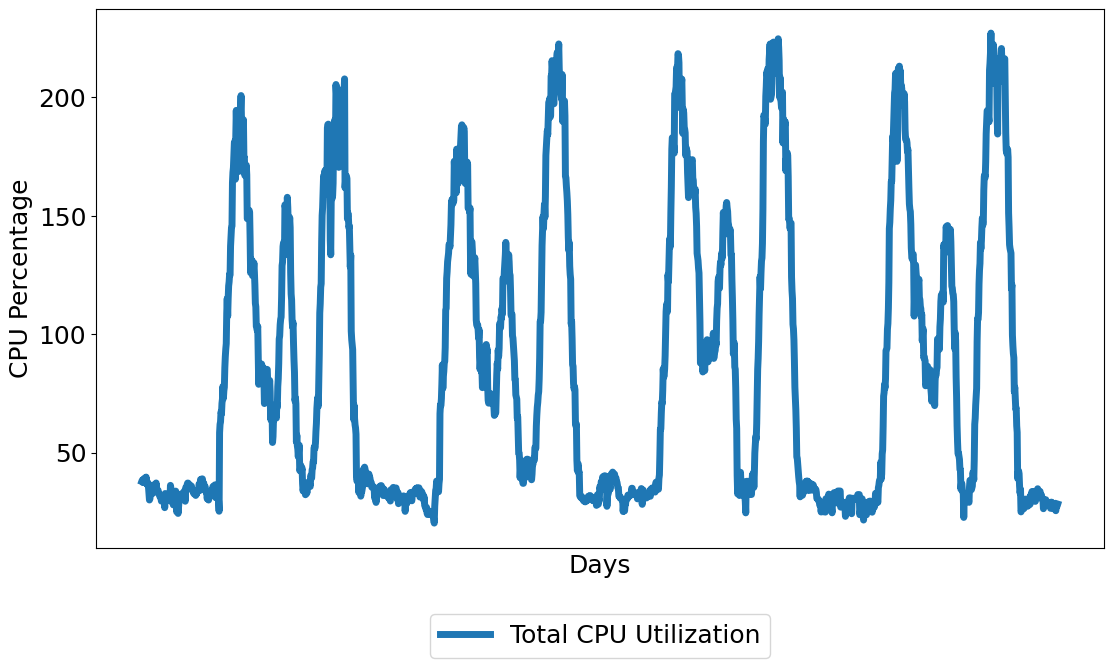
\includegraphics[width=1.0\linewidth]{Figures/LSTM-Initial-Data.png}
\end{figure}

This data has two major peaks during the morning and evening, with one smaller peak in the afternoon. The night time workload is consistently minimal. Due to the randomness included in the algorithm, each of the peaks are never the exact same, which helps mimic the real data an edge architecture would experience. However, this data has several abrupt changes every few minutes, for example the utilization could be 100\% at 5:00pm, then suddenly drop down to 75\% at 5:10pm, before coming back up to 110\% at 5:20pm. These abrupt changes makes it difficult for the LSTM to be able to accurately predict the future workloads, and requires a much larger input sequence to reduce model loss, which can significantly drive up training times.\par

To get around this issue, the proactive autoscaler introduces a data pre-processing component. This involves the use of noise reduction and data smoothing algorithm. This is done through a popular technique known as the Savitzky-Golay filter \cite{savitzky1964smoothing}. This filter takes $N$ points in a given time-series, with a filter width $w$, and calculates a polynomial average of order $o$ \cite{schafer2011savitzky}. The resulting time-series data which can be seen in figure \ref{fig:lstm-smooth-data} has considerably less deviations between consecutive points, and devoid of noise.\par

\begin{figure}[htb]
    \centering
    \caption{Example of pre-processed workload}
    \label{fig:lstm-smooth-data}
    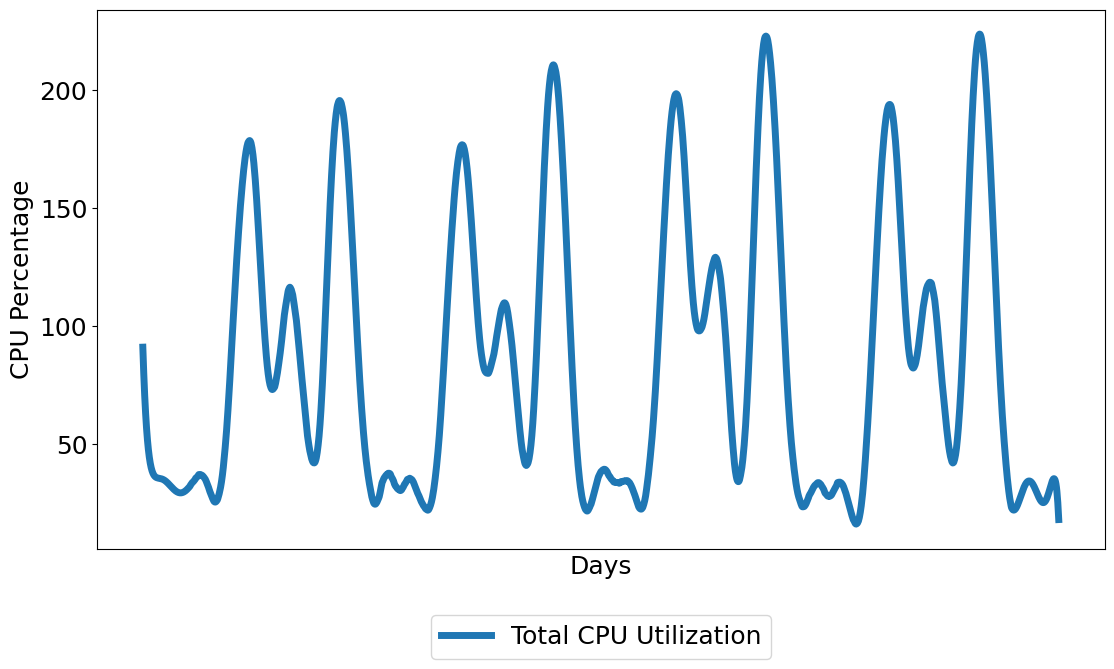
\includegraphics[width=1.0\linewidth]{Figures/LSTM-Smooth-Data.png}
\end{figure}

The filtered data is then normalized, and is then ready to be used to trained the model. Alongside the architecture configured in table \ref{tab:lstm-layers}, the LSTM model contains the following default hyper-parameter values depicted in table \ref{tab:lstm-params}.

%TC:ignore
\begin{table}
    \caption{Proactive forecaster hyper-parameter values.}\label{tab:lstm-params}
    \centering
    \begin{tabular}{|l|l|l|}
        \hline
        Hyper-parameter & Value\\
        \hline
        $learning\_rate$ & 0.005\\
        $epochs$         & 75\\
        $batch\_size$    & 100\\
        $optimizer$      & Adam \cite{diederik2014adam}\\
        \hline
    \end{tabular}
\end{table}
%TC:endignore

The parameters are chosen in such a way that they minimize training time and over-fitting, while maximizing prediction accuracy. To further reduce over-fitting, an additional function known as ``early-stop'' is defined which halts the training of the model if the loss does not decrease for 10 consecutive epoch iterations. These parameters were determined based on the research experiments conducted by Siami-Namini et al. \cite{siami2018comparison}.\par

\begin{center}
    \captionof{figure}{Loss and root mean squared error per training epoch}
    \label{fig:loss-mse-training}
    \begin{tikzpicture}[scale=0.5]
        \begin{axis}
            \addplot table [x=Step, y=Value, col sep=comma] {Data/epoch_loss.csv};
        \end{axis}
    \end{tikzpicture}
    \qquad
    \begin{tikzpicture}[scale=0.5]
        \begin{axis}
            \addplot table [x=Step, y=Value, col sep=comma] {Data/epoch_root_mean_squared_error.csv};
        \end{axis}
    \end{tikzpicture}
\end{center}

Figure \ref{fig:loss-mse-training} shows how the loss and root mean squared error of the model decreases with respect to the training epochs. The loss drops drastically for the first 25 epochs, before reducing gradually until the $60^{th}$ epoch. From here until the end of training, the loss value plateaus, making the limited gains too costly in terms of training time. From this, the choice of 75 epochs for the model training is justified.\par

A similar trend is seen in the weights and biases of the LSTM. Figure \ref{fig:bias-weight-training} shows how these values for the final dense layer change over each epoch. In the first epoch, the biases are uniformly distributed, but slowly converge to a smaller value. Similarly, the final layer weights are more evenly distributed on the final epoch.\par

\begin{figure}[htb]
    \centering
    \caption{Training bias and weights per training epoch}
    \label{fig:bias-weight-training}
    \begin{minipage}{0.45\linewidth}
        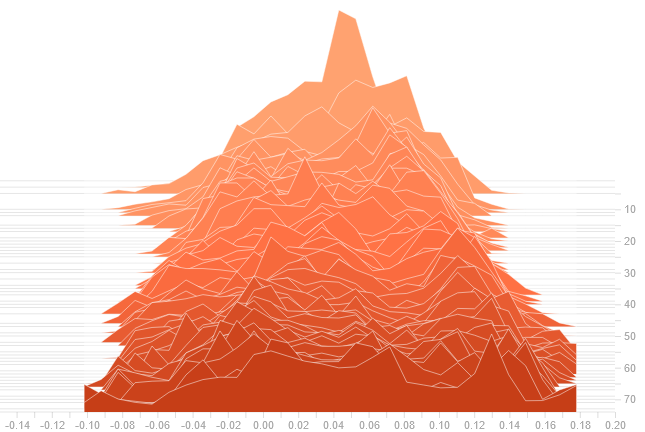
\includegraphics[width=1.0\linewidth]{Figures/LSTM-Bias.png}
    \end{minipage}\hfill
    \begin{minipage}{0.45\linewidth}
        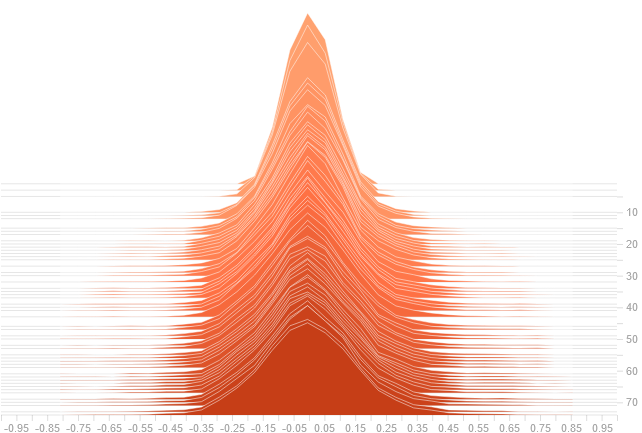
\includegraphics[width=1.0\linewidth]{Figures/LSTM-Weights.png}
    \end{minipage}
\end{figure}

The model training, validation and comparison with previous model performances takes approximately 3 minutes, after which, the model predicts the subsequent day's forecast. Figure \ref{fig:lstm-final-data} shows how this looks. The forecaster accurately depicts the initial peaks for the entire day. However, the rest of the data may not be as accurate, however this is not a significant drawback for the hybrid model, as the reactive algorithm is capable of making minor adjustments.

\begin{figure}[htb]
    \centering
    \caption{Example of the forecasted workload}
    \label{fig:lstm-final-data}
    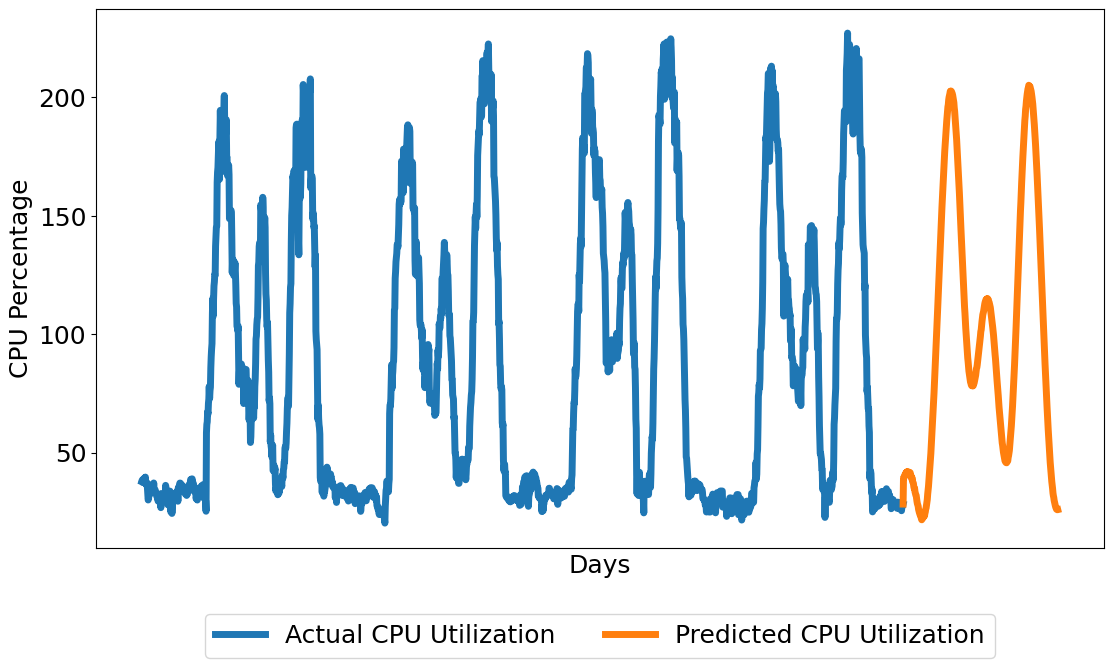
\includegraphics[width=1.0\linewidth]{Figures/LSTM-Final-Data.png}
\end{figure}

\subsection{Autoscaler Daemon}
\label{subsec:ch4-auto-daemon-subsection}

The autoscaler daemon stores a maximum of seven days of data for use by the proactive forecaster. Data that is too old is not very useful for a time-series model training on semi-predictable data \cite{greff2016lstm}, and only increases training time without adding much to the accuracy. This data is refreshed every 15 seconds to ensure that the latest data is always available to the hybrid autoscalers.\par

The daemon sends a training request to the proactive autoscaler once every night. The time is chosen so that, due to the low resource usage, the training process can claim as much of the edge resources as possible without affecting the network availability. However, before sending the request, the daemon computes whether or not an SLA violation took place in the past 24 hours or not. If it detects a violation, it assumes that the forecaster has not learnt enough of the time-series due to a variety of reasons such as lack of training data or conservative parameter values. To counteract this, the daemon performs the following corrections:

\begin{itemize}
    \item $learning\_rate$ is decreased by 0.0005, to a minimum value of 0.002.
    \item $epochs$ is increased by 5, to a maximum of 100.
    \item $batch\_size$ is increased by 10, to a maximum of 200.
    \item $early\_stop$ threshold is increased by 5, to a maximum of 25.
\end{itemize}

The assumption here is the training accuracy can be kick started by sacrificing training time for one duration to better learn the time series features and thus reduce SLA violations. As long as SLA violations occur, these modifications keep being performed up until their configured limits. Experimental testing demonstrated that, at the most extreme hyper-parameter configuration, the training time increases to 10 minutes. Once no SLA violations are detected in a day, the hyper-parameters are reverted back to default. Doing so does not cause the model to lose any previous learnings, but has the added benefit of reducing training time and resources once again.
\clearpage

\def\chaptertitle{Performance Evaluation}

\lhead{\emph{\chaptertitle}}

\chapter{\chaptertitle}
\label{ch:performance-evaluation}

In this chapter, we begin by discussing the underlying hardware configuration, and assumptions made before beginning the auto-scaling experiments in section \ref{sec:ch5-hardware-assumptions}. The cluster configuration, which involves the resource divisions between servers, overall cluster architecture, and deployment resources is discussed in section \ref{sec:ch5-cluster-config}.

\section{Assumptions and Underlying Hardware}
\label{sec:ch5-hardware-assumptions}

For the hardware setup, servers in the Melbourne Research Cloud \footnote{\url{https://docs.cloud.unimelb.edu.au/}} were leveraged to deploy microservices on. The set up consisted of 6 servers, using a total of 16 CPU cores and 48GB of memory. These servers were separated into a cloud and edge layer. The servers on the cloud layer have a significantly higher amount of CPU cores and memory assigned compared to the servers in the edge layer, to simulate the scarcity of resources in the edge layer. Furthermore, a simulated latency was added between inter-layer server communication to mimic the perceived distance between edge nodes and large data-centres.\par

Each server consists of an Ubuntu 22.04 operating system. Kubernetes v1.28.2 is used as the container orchestration technology behind the experimental micro service setup. For maximum flexibility, a bare-metal implementation of Kubernetes is used, instead of ready made solutions available from Amazon or Google. The control plane is deployed on the cloud layer, while the data plane is on the edge layer. Furthermore, several assumptions were made before proceeding with the experimentation:

\begin{itemize}
    \item The only auto-scaling performed would be horizontal pod auto-scaling. Vertical and cluster auto-scaling were out of scope of the project.
    \item The pods on which auto-scaling are not applied will have the maximum possible resource allocation to remove the chances of bottleneck.
    \item At no point in the experiment would a node be taken down, or new node be added.
    \item The autoscaler assumes that every node in the edge layer is an equally likely candidate for scheduling pods on.
\end{itemize}

\section{Cluster Configuration}
\label{sec:ch5-cluster-config}

The hardware was divided into the cloud and edge layer as depicted in table \ref{tab:cluster-hw-overview}. The control plane was divided into two servers, one for handling the Kubernetes control plane scheduling, API service, and etcd deployments, and the other for storing the Prometheus database, along with the microservice Jaeger metrics collection. The edge layer consisted of four servers with far less resources, to depict the difference in computing power. The network layer between the edge and cloud deployments also contained a simulated latency to denote the perceived geographical distance between them.\par

%TC:ignore
\begin{table}
    \caption{Cluster architectural layout}\label{tab:cluster-hw-overview}
    \centering
    \begin{tabular}{|l|l|l|l|}
        \hline
        Node & Layer & CPU (cores) & Memory (GB)\\
        \hline
        Control-Plane-K8s & Cloud & 4 & 16\\
        Control-Plane-DB  & Cloud & 4 & 16\\
        Data-Plane-1      & Edge  & 2 & 4\\
        Data-Plane-2      & Edge  & 2 & 4\\
        Data-Plane-3      & Edge  & 2 & 4\\
        Data-Plane-4      & Edge  & 2 & 4\\
        \hline
    \end{tabular}
\end{table}
%TC:endignore

The cloud and edge nodes were differentiated in through Kubernetes through the internal labelling system. A key ``type'' with value either ``cloud'' or ``edge'' was added to each node. This would enable the scheduler to automatically consider restricting the deployment of pods to particular nodes. For example, the Prometheus deployment would only be deployed on the node of type cloud. This process is known as ``node affinity'' \cite{santos2019towards}.\par

There were several options to deploy the social media application to Kubernetes. Manually cloning them from the repository, creating the custom resource definitions (CRDs), and deploying the YAML files is an option which gives maximum flexibility, but is difficult to debug if things go wrong. Due to this, the Kubernetes package manager Helm was used. Helm \footnote{\url{https://helm.sh/}} is another open-source project whose primary goal involved streamlining the installation, maintenance, and removal of Kubernetes deployments. This is achieved through the use of a Helm chart, which details the configuration of the project, and how to update and access it.\par

Therefore the social media application was the first to be deployed on Kubernetes. However, before deploying the application, the primary deployments to be tested needed to be configured. Based on the ``wrk2'' benchmark that was discussed above, two APIs were identified. One was a GET call to the user's home timeline, and the other was a POST method made by the user to create a post.\par

First, a default social media deployment was installed using the helm command below:

\begin{lstlisting}[
  caption={Social network installation using Helm},
  captionpos=t,
  label={lst:social-network-helm-install},
  language=bash
]
$ helm install social-media \
/DeathStarBench/socialNetwork/helm-chart/Chart.yaml -n default
\end{lstlisting}

With the social media network now deployed, a workload for both GET and POST commands were invoked to generate the latency trace on Jaeger, as depicted in listing \ref{lst:wrk2-api-calls}.

\begin{lstlisting}[
  caption={Social network installation using Helm},
  captionpos=t,
  label={lst:wrk2-api-calls},
  float=ht,
  language=bash
]
$ WRK2="/DeathStarBench/wrk2/wrk -D exp -t 1 -c 1 -d 1 -L -s -R 1"
$ HT=./wrk2/scripts/social-network/read-home-timeline.lua
$ CS=./wrk2/scripts/social-network/compose-post.lua
$ IP=$(kubectl get svc nginx-thrift --template '{{.spec.clusterIP}}')
$ PORT=8080
$ $WRK2 $HT http://$IP:$PORT/wrk2-api/home-timeline/read
$ $WRK2 $HT http://$IP:$PORT/wrk2-api/post/compose
\end{lstlisting}

With the traces generated, the deployments which require autoscaling could be identified for each. From the Jaeger traces generated in figure \ref{fig:ht-cp-trace}, it is clear that the two deployments highlighted in purple, namely ``home-timeline-service'', and ``compose-post-service'', were the major bottlenecks in API processing, and thus required autoscaling. Therefore, the helm deployment was updated to assign resources to them. The resources were assigned in a realistic manner consistent with edge deployments, and based on the number of components each deployment answered to. Listing \ref{lst:deploy-resource-update} shows the CPU resources assigned to both deployments.\par

\begin{figure}[htb]
    \centering
    \caption{Home Timeline and Compose Post API trace}
    \label{fig:ht-cp-trace}
    \begin{minipage}{0.25\linewidth}
        %\caption{Home Timeline API trace}
        %\label{fig:home-timeline-trace}
        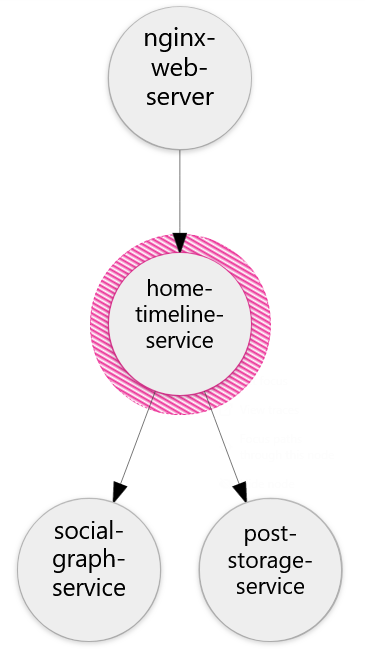
\includegraphics[width=1.0\linewidth]{Figures/Home-Timeline-GET-Trace.png}
    \end{minipage}\hfill
    \begin{minipage}{0.75\linewidth}
        %\caption{Compose Post API trace}
        %\label{fig:compose-post-trace}
        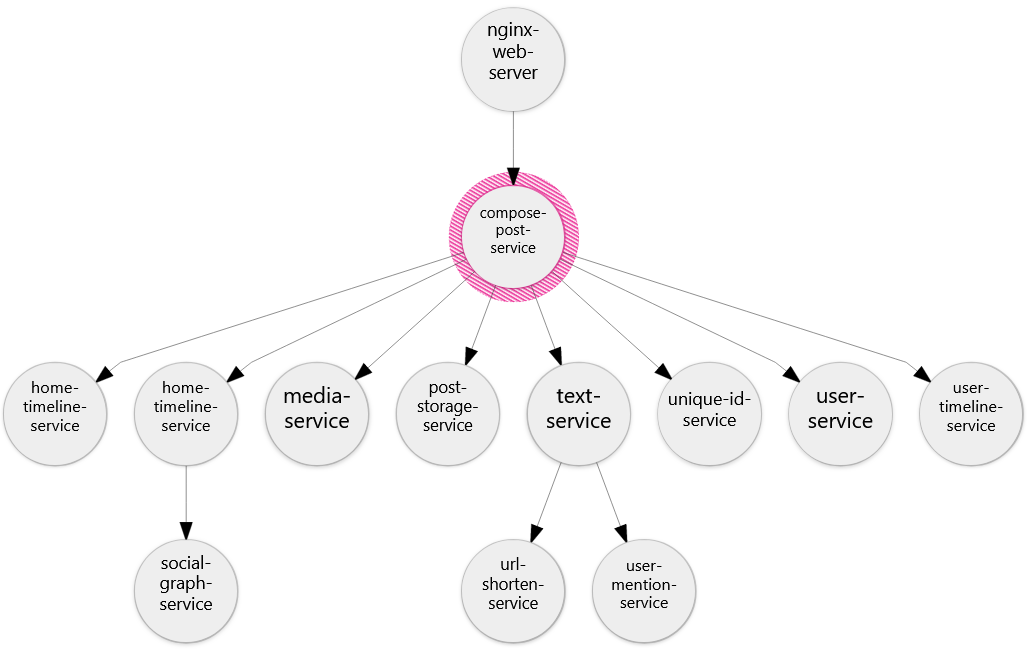
\includegraphics[width=1.0\linewidth]{Figures/Compose-Post-POST-Trace.png}
    \end{minipage}
\end{figure}

\begin{lstlisting}[
  caption={Update resources for bottlenecked deployments},
  captionpos=t,
  label={lst:deploy-resource-update},
  language=bash
]
$ helm upgrade social-media \
/DeathStarBench/socialNetwork/helm-chart/Chart.yaml -n default \
--set-string compose-post-service.container.resources="requests: 
      cpu: "30m"
    limits:
      cpu: "30m"" \
--set-string home-timeline-service.container.resources="requests: 
      cpu: "15m"
    limits:
      cpu: "15m""
\end{lstlisting}

\section{Experiment Setup}
\label{sec:ch5-exp-setup}

Two independent experiments were conducted to verify the performance of the hybrid autoscaler. The social media application was first tested using the GET API to autoscale the home-timeline-service deployment. Then, a more demanding as well as challenging workload was applied to the POST API for autoscaling the compose-post-service deployment. For both these experiments, the workload generation algorithm was used to create realistic daily workloads and tested over the period of one week. Both experiments would configure a flexible SLA latency agreement to be maintained. For the first experiment, the SLA constraint was set to a 150 milliseconds latency, and for the second experiment, it was 1000 milliseconds. The flexible SLA constraint was the primary focus of the experiment, however a moderate and strict SLA constraint was also chosen and tested. The SLA values are shown in table \ref{tab:experiment-sla-values}.\par

%TC:ignore
\begin{table}
    \caption{Experimental SLA constraints}\label{tab:experiment-sla-values}
    \centering
    \begin{tabular}{|l|l|l|}
        \hline
        SLA Type & GET API constraint (ms) & POST API constraint (ms)\\
        \hline
        Flexible    & 150   & 1000\\
        Moderate    & 125   & 900\\
        Strict      & 100   & 800\\
        \hline
    \end{tabular}
\end{table}
%TC:endignore

For the proposed hybrid algorithm to achieve these autoscaling goals within the SLA constraints, the autoscaling subsystems were configured as follows. The reactive autoscaler would check if the CPU utilization of the deployment was exceeding the 50\% threshold. If so, it would scale up based on the cooldowns and tolerations set. The proactive autoscaler on the other hand would check if the forecasted CPU utilization in the next 20 minutes was going to breach the 50\% threshold, and if so, would autoscale with the same configured parameters as the reactive one. The daemon would store the total CPU utilization of the deployment as a time-series for a maximum of seven days, and constantly check for SLA violations to tweak the hyper-parameters of the forecaster as discussed above in section \ref{subsec:ch4-auto-daemon-subsection}. To measure the effectiveness of the hybrid autoscaler, three baseline algorithms were chosen for comparison. All three would autoscale at the CPU threshold of 50\%. Furthermore, these algorithms would be implementations based on the ones discussed in section \ref{sec:ch2-lit-review}.\par

The first was the default Kubernetes horizontal pod autoscaler. No modifications to the configuration were made, thus the scale up cooldown was 0 seconds, while the scale down was 300 seconds. Additionally, the autoscaler had no knowledge of the workload distribution or SLA violations on the edge nodes.\par

The second baseline was an implementation of the reactive traffic aware horizontal pod autoscaler created by Phan et al. \cite{phan2022traffic}. This autoscaler scheduler would compute the ratio of workloads being exerted on the different edge nodes with the deployment pods. Once it did so, it would scale these resources in a commensurate proportion.\par

Finally, the last baseline implementation was the Proactive Pod Autoscaler (PPA) devised by Ju et al. \cite{ju2021proactive}. This algorithm was an open-ended implementation which enabled the user to plugin a deep learning model of their choice. The PPA architecture consisted of three sub-sections, the formulator, evaluator, and updater. An LSTM model was injected into the autoscaler as the model file. This LSTM implementation was similar to the one used in the hybrid autoscaler, however it differed in two key elements. First, the LSTM did not expect pre-processed data without noise, and thus dealt with more complex time-series data. Secondly, due to this additional computation, the LSTM contained a deeper architecture layer with more neural network units. This was required as the algorithm had to correctly predict the complete future workload since there was no reactive autoscaler to fall back on. Over a fixed interval, the algorithm continuously looped through the time-series data and saved the forecast result to a metrics file. The evaluator took these outputs from the metrics file, along with the LSTM from the model file to predict the number of pods to assign in advance, and requested the Kubernetes scheduler for scaling through the API Service. A second loop, known as the update loop, then updated the LSTM model using the latest forecast, and cleared the metrics file. The hyper-parameters were carefully tuned to ensure that the model did not under-perform too significantly. Finally, the PPA architecture did not take into account SLA compliance, and thus SLA metrics were not provided as a feedback for hyper-parameter tuning.\par



\clearpage

\def\chaptertitle{Conclusion}

\lhead{\emph{\chaptertitle}}

\chapter{\chaptertitle}
\label{ch:conclusion}

\section{Contributions}
\label{sec:ch6-contributions}

\section{Future Work}
\label{sec:ch6-future-work}

\subsection{Current Limitations}
\label{subsec:ch6-limitations}

\subsection{Proposed Extensions}
\label{subsec:ch6-extensions}

\subsubsection{Multi-Parameter Forecaster}
\label{subsubsec:ch6-multi-param}

\subsubsection{Autoregressive Forecaster}
\label{subsubsec:ch6-multi-param}

\subsubsection{Multi-SLA Constraints}
\label{subsubsec:ch6-multi-sla}

\subsubsection{Advanced LSTM Configurations}
\label{subsubsec:;ch6-advanced-lstm-config}


\addtocontents{toc}{\vspace{2em}}

%TC:ignore
\appendix
%\input{appendices/data.tex}
%\input{appendices/programs.tex}
\chapter{Appendix}

%TC:endignore

\addtocontents{toc}{\vspace{2em}}
\backmatter

\lhead{\emph{Bibliography}}
\bibliographystyle{unsrtnat}
\bibliography{Thesis}
\label{bibliography}

\end{document}
